\pdfoutput=1

\documentclass[11pt]{article}

\usepackage[]{acl}

\usepackage{times}
\usepackage{latexsym}

\newcommand{\fan}[1]{\textcolor{blue}{\bf\small [#1 --Fan]}}


\definecolor{snsblue}{HTML}{4c72b0}
\definecolor{snsorange}{HTML}{dd8452}
\definecolor{snsgreen}{HTML}{66c2a5}
\definecolor{snslightorange}{HTML}{fc8d62}
\usepackage[T1]{fontenc}

\usepackage[utf8]{inputenc}

\usepackage{microtype}
\usepackage{booktabs} 
\usepackage{multirow}
\usepackage{inconsolata}
\usepackage{colortbl}
\usepackage{xcolor}          
\usepackage{amssymb} 
\usepackage{subcaption}
\usepackage{subfloat}
\usepackage{graphicx}
 \usepackage{amsmath}
\newcommand\sect[1]{\S\ref{#1}}
\newcommand{\priortodo}[1]{{\color{blue} [TODO: #1]}}
\newcommand{\kaiser}[1]{{\color{cyan} [Kaiser: #1]}}
\newcommand{\saleh}[1]{{\color{green} [Saleh: #1]}}
\newcommand{\niyati}[1]{{\color{teal} [Niyati: #1]}}
\newcommand{\carlos}[1]{{\color{purple} [Carlos: #1]}}

\usepackage{tablefootnote}

\title{Amuro \& Char: Analyzing the Relationship between \\ Pre-Training and Fine-Tuning of Large Language Models}

 \author{Kaiser Sun \quad Mark Dredze \\
 Johns Hopkins University
 \\ Baltimore, MD USA \\
\texttt{\{hsun74,mdredze\}@cs.jhu.edu}\\
}

\begin{document}
\maketitle
\begin{abstract}
\begin{abstract}
Diffusion Models have emerged as powerful generative models for high-quality image synthesis, with many subsequent image editing techniques based on them. However, the ease of text-based image editing introduces significant risks, such as malicious editing for scams or intellectual property infringement. Previous works have attempted to safeguard images from diffusion-based editing by adding imperceptible perturbations. These methods are costly and specifically target prevalent Latent Diffusion Models (LDMs), while Pixel-domain Diffusion Models (PDMs) remain largely unexplored and robust against such attacks. Our work addresses this gap by proposing a novel attacking framework with a feature representation attack loss that exploits vulnerabilities in denoising UNets and a latent optimization strategy to enhance the naturalness of protected images. Extensive experiments demonstrate the effectiveness of our approach in attacking dominant PDM-based editing methods (e.g., SDEdit) while maintaining reasonable protection fidelity and robustness against common defense methods. Additionally, our framework is extensible to LDMs, achieving comparable performance to existing approaches.
\end{abstract}

\end{abstract}


\section{Introduction}



The rise of large language models (LLMs) as a general-purpose tool for a diverse range of natural language processing tasks has dramatically transformed the field, introducing new paradigms for data collection and model training 
(\citealp{brown2020language}, \citealp{biderman2023pythia}, \citealp{touvron2023llama}, 
\citealp{jiang2023mistral}, 
\citealp{chowdhery2023palm}, \citealp{groeneveld2024olmo}, \citealp{wang2024helpsteer2}, \textit{inter alia}).
Numerous models, training methods, datasets, and evaluation methods continue to be developed on an ongoing basis.
Nevertheless, a unified paradigm has emerged for training LLMs: pre-train on an enormous corpus of diverse documents, ranging from 250B \cite{biderman2023pythia} to 15T \cite{llama3modelcard} tokens, followed by an alignment stage to make the model more useful and performative for various tasks.

\twocolumn[{%
	\renewcommand\twocolumn[1][]{#1}%
	\maketitle
	\begin{center}
		\newcommand{\teaserwidth}{\textwidth}
		% \vspace{-0.15in}
		\centerline{
			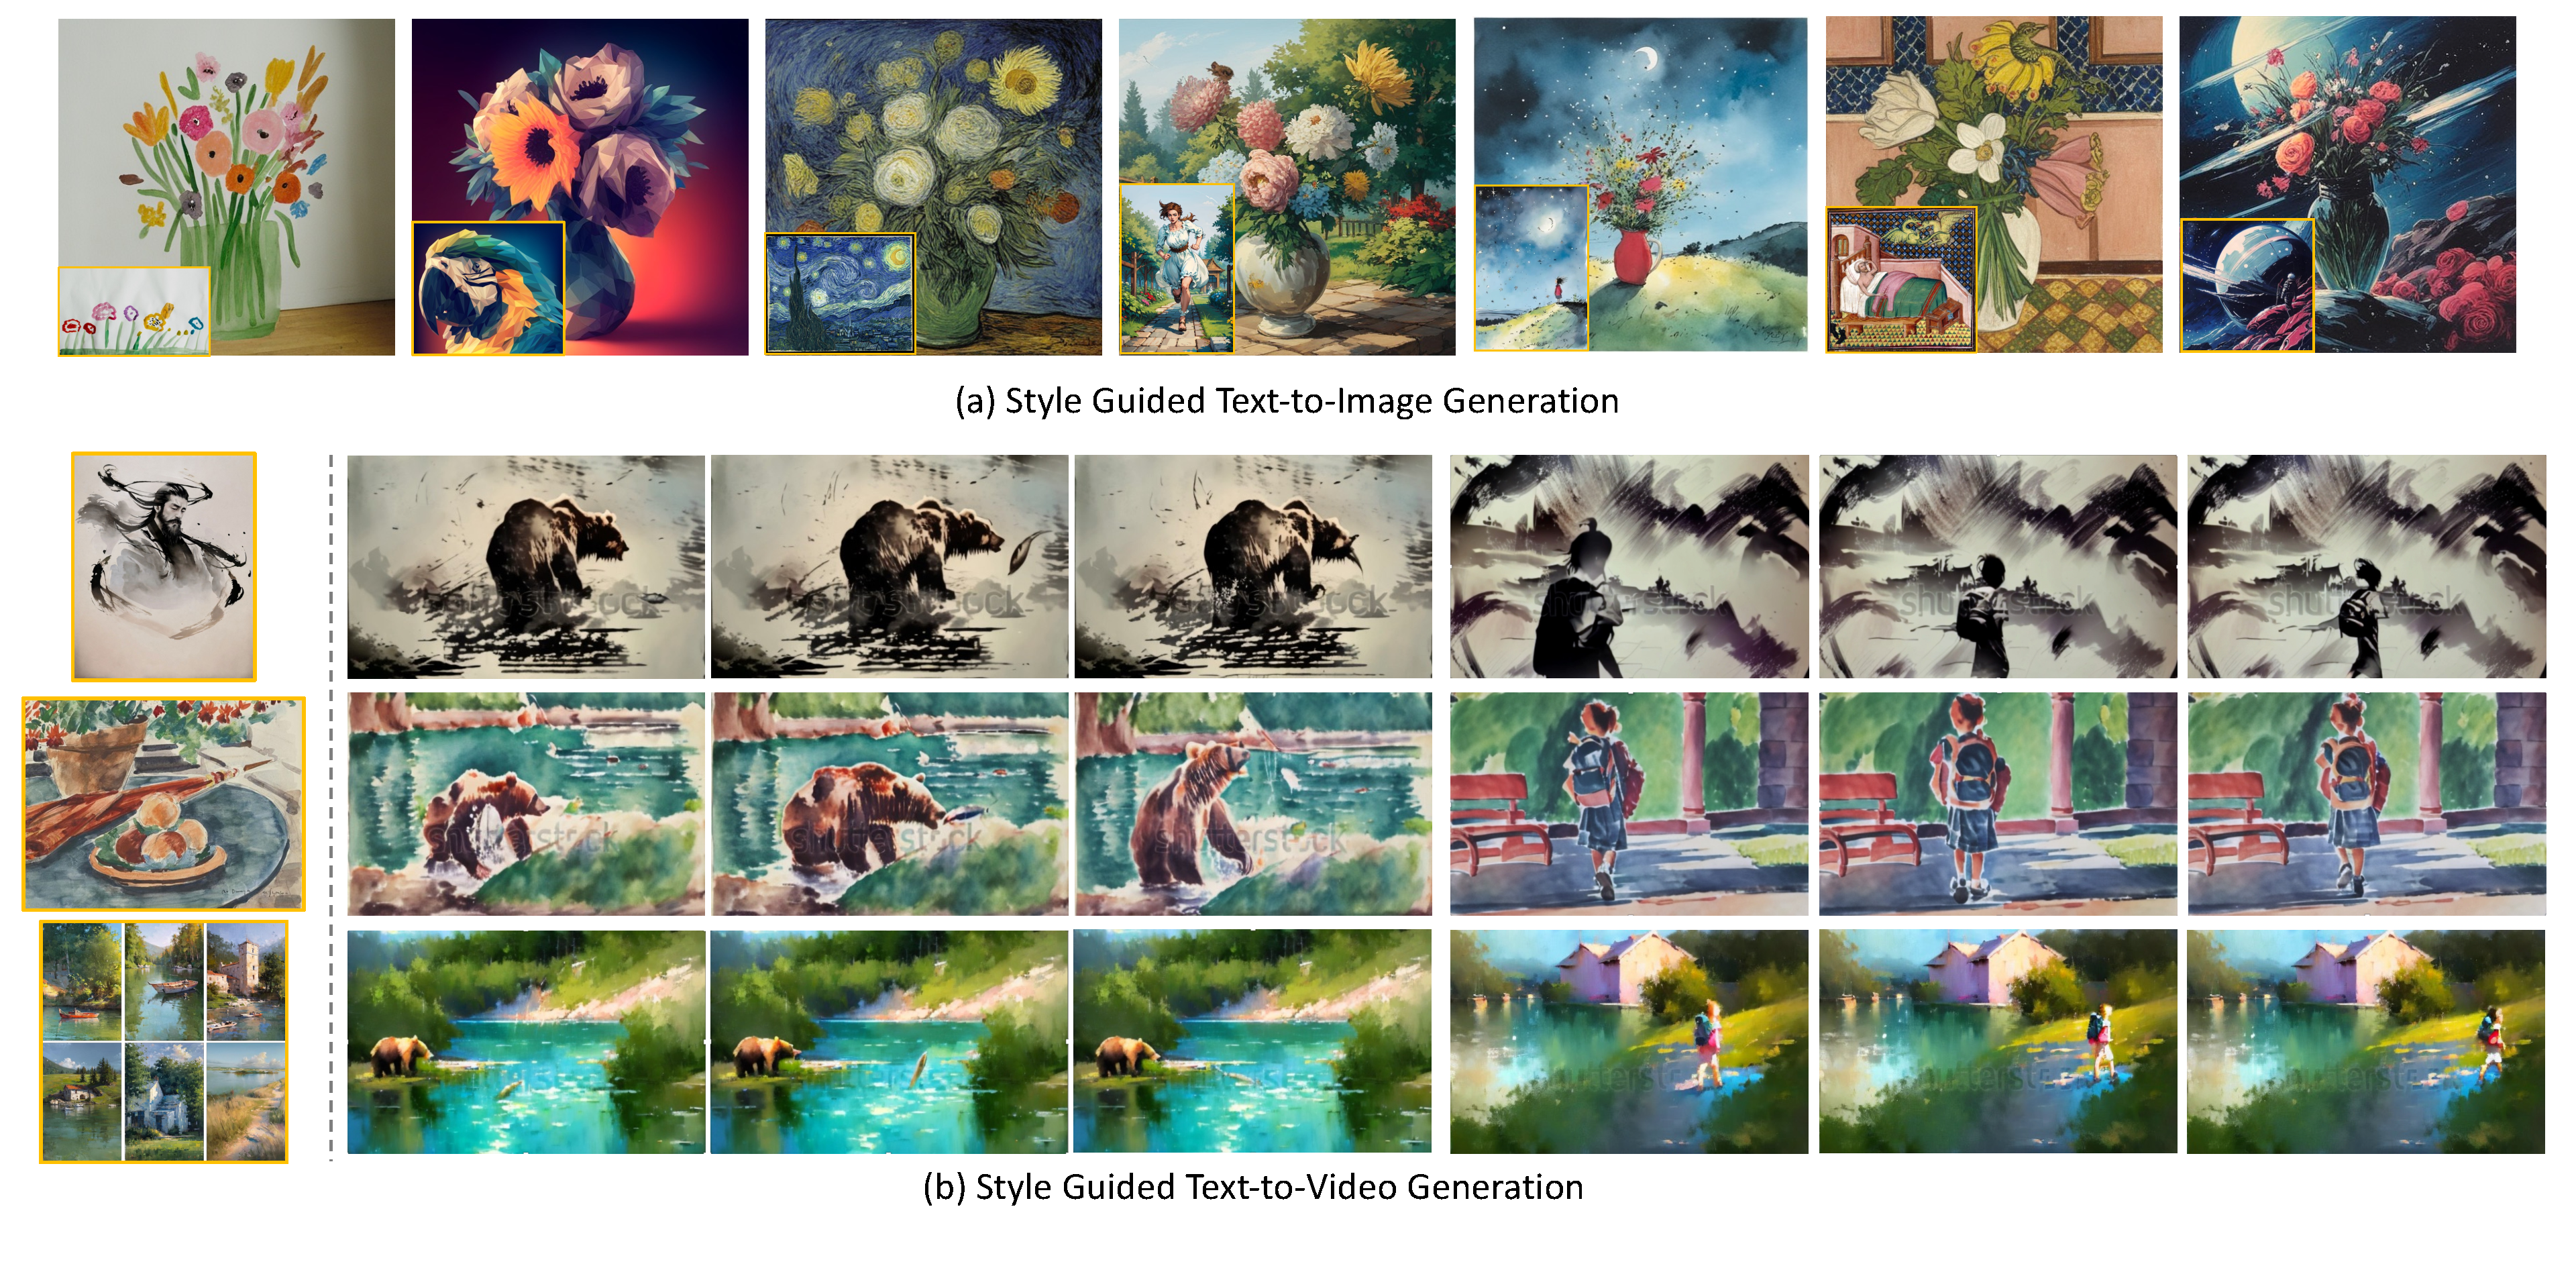
\includegraphics[width=\teaserwidth,clip]{figures/pdf_files/teaser.pdf}
		}
		\vspace{-1ex}
		\captionof{figure}{\textbf{Human Gaussian Splats (\acronym)} is a neural rendering framework that trains on 50-100 frames of a monocular video containing a human in a scene. HUGS enables novel view rendering with novel human poses at 60 FPS by learning a disentangled representation that can also render the human in other scenes. }
		% \vspace{-0.08in}
		\label{fig:teaser}
	\end{center}%
}]
Based on this paradigm, work has focused on improving these two stages. 
Work to improve pre-trained models includes larger training sets \cite{hoffmann2022training, llama3modelcard, touvron2023llama}, different data selection mechanisms \cite{xia2024less}, higher quality data \cite{zhou2024lima}, and various model architectures \cite{su2024roformer, touvron2023llama}. 
Meanwhile, research on model alignment includes different training objectives \cite{rafailov2024direct, schulman2017proximal},
new datasets \cite{narayanan-aepli-2024-tulu-resource}, more efficient training \cite{hu2021lora,dettmers2024qlora} and safety tuning \cite{bianchi2023safety}. The alignment stage usually involves either supervised fine-tuning for specific tasks or instruction fine-tuning for general-purpose usage. 
Regardless, fine-tuning (almost always) comes at the end of pre-training and yields remarkable improvements on downstream tasks \cite{touvron2023llama, groeneveld2024olmo}. 
Consequently, the benefits of each stage are largely explored independently, with improvements to pretraining being orthogonal to benefits from model alignment.

Rather than explore these two training regimes independently, we question: {\bf how do model pretraining and fine-tuning interact to affect the resulting model?} Does more pre-training hinder better fine-tuning results? What does the model learn and forget during pre-training as well as fine-tuning?
Answering these questions requires us to examine how models learn during pre-training and how this affects fine-tuning. Therefore, 
we fine-tune {\bf multiple pre-training checkpoints} of a large language model (Figure~\ref{fig:experiment-illu}), evaluating each checkpoint and its fine-tuned version on downstream evaluation sets.
We track model abilities during pre-training and compare them to improvements achievable after fine-tuning at the corresponding pre-training step.
We explore both supervised and instruction fine-tuning, testing the models' memorization and forgetting when learning specific tasks and serving as general-purpose language-AI tools. 
To the best of our knowledge, we are the first to explore fine-tuning intermediate model checkpoints.

Our experiments yield insights into LLM training.
We find that (1) continued pre-training can improve a model in ways that are only revealed after fine-tuning (\sect{sec:finding:PTFT}); (2) tasks for which the model already performs well during pre-training benefit much less from fine-tuning than those where the model does not demonstrate capabilities (\sect{sec:finding:base-eval}, \sect{sec:finding:PTFT}); (3) although supervised fine-tuning can improve performance on in-distribution tasks, it can also cause the model to forget domain knowledge or tasks that it was previously capable of solving (\sect{sec:finding:what}); (4) fine-tuned models show high sensitivity to evaluation prompts, but this sensitivity can be alleviated by more pre-training (\sect{sec:finding:what}).
Our findings provide insights into model training and can inform methods for both pre-training and fine-tuning. Furthermore, our work shows the value of analyzing the training dynamics, in addition to analyzing the final LLM, as an aspect of interpretability, and we encourage model developers to release these checkpoints to aid future studies.


\section{Background: Model Training}

We begin with a brief survey of the core components of LLM training: pre-training, fine-tuning, and instruction fine-tuning. 
We also discuss the related topic of in-context learning as well as different efficient fine-tuning strategies.

We use ``model alignment'' as a general term for techniques that align a model with a desired behavior, which can be accomplished by fine-tuning models after pretraining. The term is also associated with other definitions \cite{shen2024bidirectional}. 
We also note several related studies that explore training dynamics to understand model behavior \cite{tirumala2022memorization, chen2023sudden, tian2023scan}.
With this in mind, we conduct an empirical study on how the amount of pre-training affects the effectiveness of fine-tuning.

\paragraph{Pre-training}
The first step of training a LLM is pre-training on a massive text corpus
 \cite{achiam2023gpt, touvron2023llama, groeneveld2024olmo}.
For decoder-only models in the GPT family, the subject of our paper, work since the introduction of GPT-2 \cite{radford2019language} has focused on scaling up model training. 
Initial work increased model size to hundreds of billions of parameters \cite{brown2020language, rae2021scaling, chowdhery2023palm}, along with explorations in model size, training corpus size, and training data characteristics \cite{hoffmann2022training, gururangan-etal-2020-dont}. 
Since the push towards large models, work has shifted to increasing the amount of pre-training data \cite{together2023redpajama, soldaini2024dolma}, with new models now reaching 15 trillion tokens \cite{llama3modelcard}. 
Studies of model performance on various tasks at different model sizes introduced the idea of emergent model abilities \cite{wei2022emergent}, with new model abilities being revealed as model training grows.

We also recognize a particularly important trend for this paper: model openness. 
Early LLMs were proprietary models accessible only through an API. 
The first large open model, Bloom \cite{bloom-strom-etal-2023-preparing}, allowed widespread LLM evaluation. 
Subsequent open models, such as OPT \cite{zhang2022opt}, LLaMA \cite{touvron2023llama,keles-bayrakli-2024-llama-2} and others \cite{biderman2023pythia, openlm, almazrouei2023falcon}, have become the norm. 
In this paper, we study OLMo \cite{groeneveld2024olmo}, one of the only models to release individual pre-training checkpoints.

\paragraph{Fine-Tuning}
Early work on instruction fine-tuning using reinforcement learning with human feedback (RLHF) \cite{ziegler2019fine, stiennon2020learning, ouyang2022training} demonstrates the dramatic effect that model alignment could have on a pre-training model. 
When a specific task of interest has been identified, supervised fine-tuning can improve a pre-trained model. 
Task-agnostic tuning became popularized with the advent of T5 models \citep{raffel2020exploring}, where a pre-trained LLM is tuned using a general text-to-text solution. 
When multiple tasks are given to the model, the model is commonly given a task-specific prefix or an instruction along with the task input, leading to the development of various methods of prefix tuning \cite{li-liang-2021-prefix} and instruction tuning \cite{wei2021finetuned, mishra-etal-2022-cross, victor2022multitask}.

\paragraph{Instruction Fine-Tuning}
Instruction fine-tuning is preferred when more general model behaviors are desired. 
Popularized through reinforcement-learning with human feedback (RLHF) \cite{christiano2017deep, ziegler2019fine, stiennon2020learning, ouyang2022training} and reinforcement-learning with AI feedback (RLAIF) \cite{lee2023rlaif}, these methods utilize a reward model to simulate human feedback.
Others explore human preference tuning without a reward model \cite{rafailov2024direct, song2024preference, xu2024contrastive}, or study the effects of these tuning methods \citep{shen2024bidirectional,perez-etal-2023-discovering}.
\citet{sharma2024critical} show that supervised fine-tuning can lead to similar performance as RLAIF.

\paragraph{In-Context Learning}
While not the subject of this paper since it does not make changes to model parameters, in-context learning utilizes a small amount of supervised data to improve model performance. 
ICL, also called few-shot learning, 
is also used as an evaluation strategy where the model is given a prompt composed of examples of tasks expected to be solved. The underlying model is evaluated based on its response to the input. 
ICL can benefit from a larger context window that adds more examples, which can spur work on the development of model quantization techniques \cite{dettmers2022gpt3} and the alleviation of hardware constraints \cite{brown2020language, xie2021explanation, min-etal-2022-rethinking}.

\paragraph{Fine-Tuning Techniques}
While model pre-training can be done by a few groups with large resources interested in developing new models, fine-tuning depends on the task and is of broad interest. Therefore, many techniques facilitate time-, memory-, and data-efficient model training through parameter-efficient fine-tuning (PEFT) \cite{hu2021lora, liu2021p, liu2023gpt}, quantization \cite{jacob2018quantization, dettmers2022gpt3, dettmers2024qlora}, and specialized data filtering \cite{xia2024less, zhou2024lima, attendu-corbeil-2023-nlu}.
This paper focuses specifically on full-parameter fine-tuning, while our findings suggest the potential for data-efficient and budget-friendly training by understanding the critical turning point of model training.
Our findings are closely related to the recent study on \textit{phase transition} of model training \cite{olsson2022context, wei2022emergent, chen2023sudden}.








\section{Experimental Setup}
In this section, we describe the model and datasets used. 
The hyperparameter tuning procedure and setup for each fine-tuning setting can be found in Appendix~\ref{sec:app:hyperparameter}.

\subsection{Model Choice} 
Our paper considers OLMo-1B \cite{groeneveld2024olmo}, a high-performing open-source large language model. 
Ideally, we would evaluate multiple models, but OLMo is the only model to release intermediate pre-training checkpoints, and thus the only model that supports our analysis\footnote{\href{https://github.com/allenai/OLMo/tree/main/checkpoints/official}{https://github.com/allenai/OLMo/tree/main/checkpoints}} \footnote{We also experimented with RedPajama-INCITE (\href{https://www.together.ai/blog/redpajama-models-v1}{https://www.together.ai/blog/redpajama-models-v1}), which is the only other model to release checkpoints. After extensive experiments, we found it performed worse than OLMo, given the training data available, and did not support our analysis. Several other models claim to release training checkpoints but have not done so.}.
Despite being the only open model with training checkpoints, it fortunately has several desirable properties. First, 
the model is fully open, including the training details, pre-training data, and fine-tuning data. 
Second, the smaller model size allows us to train a model efficiently on a single A100 GPU. While evaluating a larger model would be desirable, we limit our study to the 1B model given the much larger computational demand of multi-GPU training. Our detailed analysis required significant GPU resources, which would have been prohibitive with a larger model.
We also note that OLMo-1B compares very favorably to the larger version, and recent work has shown that small models can compete with larger ones \cite{team2024gemma}.

We select model pre-training checkpoints uniformly from the pre-training history along with the first and the final checkpoints.

\subsection{Training Procedure}
We fine-tune each of the selected model checkpoints using two different procedures to create fine-tuned models: supervised fine-tuning and instruction tuning. 
The supervised fine-tuning is conducted separately for each model checkpoint and dataset, while the instructing fine-tuning is done once using the instruction dataset.
The instruction-tuned model is evaluated on a suite of LLM benchmarks.

\paragraph{Supervised Fine-tuning}
We adapt the dataset choice from \citealp{yang2024unveiling} for supervised fine-tuning. 
For each in-domain dataset, one to two cross-domain evaluation datasets are supplied.
Each pre-training checkpoint is fully fine-tuned for 3 epochs with a batch size of 8 and learning rates resulting from minimal hyperparameter tuning. 
Each task is formatted using a default prompt-completion format (Table~\ref{tab:app:promptformat}).

\paragraph{Instruction Fine-Tuning}
We instruction-tune the model on T\"{U}LU \cite{ivison2023camels}, following the decision of \citealp{groeneveld2024olmo}.
Each model checkpoint is fully fine-tuned for 5 epochs with a batch size of 8 and a learning rate of $2\times 10^{-6}$.

\begin{table}[t!]
\centering
\small
\begin{tabular}{@{}llll@{}}
\toprule
\multicolumn{4}{c}{\textbf{Supervised Fine-Tuning}} \\ \midrule
\textbf{Task} & \textbf{Training} & \textbf{ID Test} & \textbf{OOD Test} \\ \midrule
\begin{tabular}[c]{@{}l@{}}Summary \\ Generation\end{tabular} & XSum & \begin{tabular}[c]{@{}l@{}}XSum, \\ XLSum\end{tabular} & CNN \\  \arrayrulecolor{black!30}\midrule
\begin{tabular}[c]{@{}l@{}}Question \\ Generation\end{tabular} & SocialIQa & SocialIQA & \begin{tabular}[c]{@{}l@{}}SciQ, \\ TweetQA\end{tabular} \\  \arrayrulecolor{black!30}\midrule
\begin{tabular}[c]{@{}l@{}}Natural Language \\ Inference\end{tabular} & MNLI & \begin{tabular}[c]{@{}l@{}}MNLI1, \\ MNLI2\end{tabular} & \begin{tabular}[c]{@{}l@{}}RTE, \\ GPT3NLI\tablefootnote{\href{https://huggingface.co/datasets/pietrolesci/gpt3_nli}{https://huggingface.co/datasets/pietrolesci/gpt3\_nli}} \end{tabular} \\  \arrayrulecolor{black!30}\midrule
\begin{tabular}[c]{@{}l@{}}Paraphrase \\ Detection\end{tabular} & Paws & Paws & \begin{tabular}[c]{@{}l@{}}QQP, \\ STS-B\end{tabular} \\ \arrayrulecolor{black}\midrule

\multicolumn{4}{c}{\textbf{Instruction Tuning}} \\ \midrule
\textbf{Dataset} & \multicolumn{3}{l}{\textbf{Description}} \\
\midrule
T\"ULU-v2 & \multicolumn{3}{l}{A mixture of instruction datasets.} \\ 


ARC & \multicolumn{3}{l}{Grade-school multiple-choice QA.}   \\
OpenbookQA &  \multicolumn{3}{l}{Open book exam QA.} \\
Hellaswag &  \multicolumn{3}{l}{Commonsense inference.} \\
BoolQ & \multicolumn{3}{l}{Reading comprehension.}  \\
SciQ & \multicolumn{3}{l}{Science exam multiple choice QA.}  \\ \arrayrulecolor{black}\bottomrule

\end{tabular}
\caption{Dataset information. For Generation tasks, ROUGE-L is used as evaluation metric, and accuracy is used for classification tasks.}
\label{tab:tasks}
\end{table}
\subsection{Evaluation}
The evaluation challenge is to select a representative number of datasets for different types of tasks to test model abilities, recognizing that each dataset requires evaluating each model checkpoint and its fine-tuned counterparts. 
We also select datasets based on the availability of in-domain and out-of-domain samples.

\paragraph{Datasets}
The datasets are summarized in Table ~\ref{tab:tasks}.
We evaluate the model with an in-domain test set and one or two out-of-domain test sets for each of the supervised fine-tuning tasks.
We conduct experiments on the tasks of summary generation \cite{narayan-etal-2018-dont, hasan-etal-2021-xl, hermann2015teaching}, question generation \cite{sap-etal-2019-social, xiong-etal-2019-tweetqa, welbl2017crowdsourcing}, natural language inference \cite{williams-etal-2018-broad, wang-etal-2018-glue, dagan2006pascal, bar2006second, giampiccolo2007third, bentivogli2009fifth}, and paraphrase detection \cite{zhang-etal-2019-paws, wang-etal-2018-glue, agirre2007semantic}.
Each training set is sub-sampled to a size of 6,000 for fair comparisons.

In instruction fine-tuning, we base our downstream evaluation settings on \citealp{groeneveld2024olmo}, as OLMo is found to have stable performance on these datasets.
The instruction-tuned models are evaluated on ARC (both \texttt{arc easy} and \texttt{arc challenge}) \cite{clark2018think}, OpenbookQA \cite{mihaylov-etal-2018-suit}, Hellaswag \cite{zellers-etal-2019-hellaswag}, BoolQ \cite{clark-etal-2019-boolq}, and SciQ \cite{welbl2017crowdsourcing}. 


\paragraph{Metrics}
We use accuracy \cite{scikit-learn} for classification tasks and \textsc{Rouge-L} \cite{lin-2004-rouge} for generation tasks.
We set the maximum amount of newly generated tokens to 5 for classification tasks and 60 for generation tasks.
Outputs are generated with greedy decoding.
For classification tasks, we experiment with both constrained decoding and logit-based predictions.
We find the best performance by selecting the label with the highest logit of its first subtoken (Appendix~\ref{app:pred_gen}).





\begin{figure*}[t!]
    \centering
    \begin{subfigure}[b]{0.47\textwidth}
    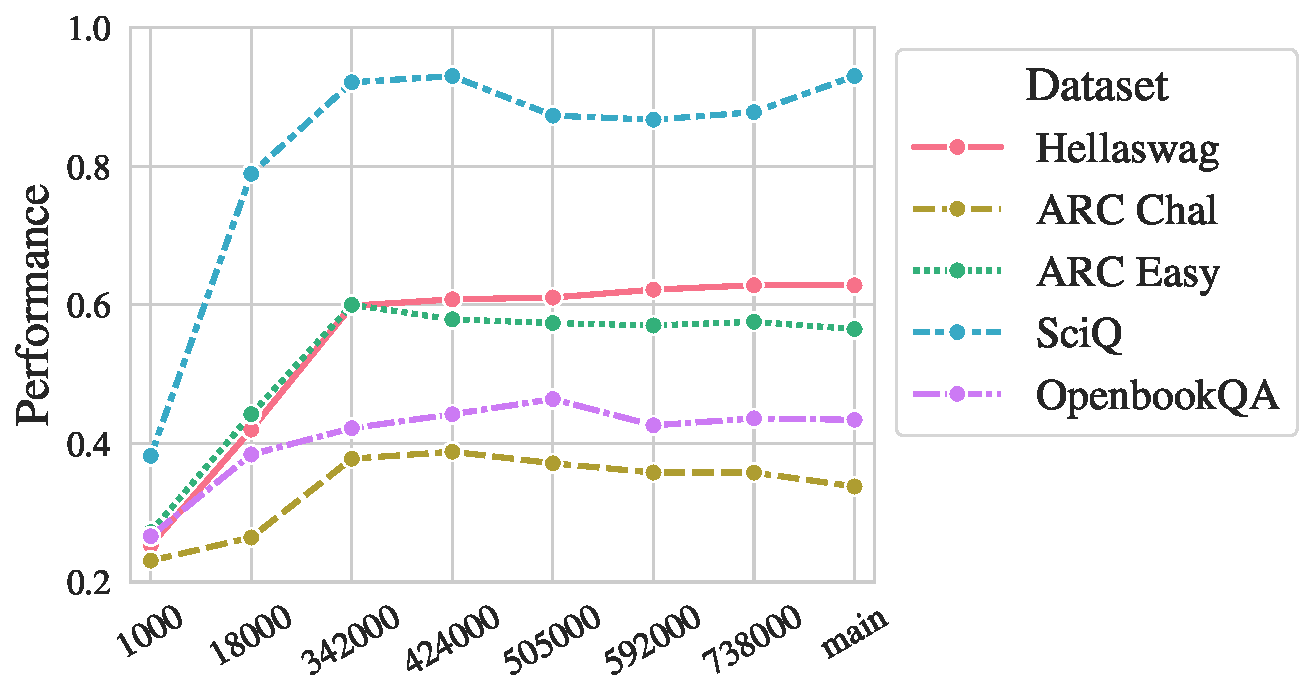
\includegraphics[width=\the\columnwidth]{figures/fig_files/base_improving.pdf}
        \caption{Learned during Pre-training.}
        \label{fig:base-eval-a}
    \end{subfigure}%
    ~ 
    \begin{subfigure}[b]{0.45\textwidth}
        \centering
    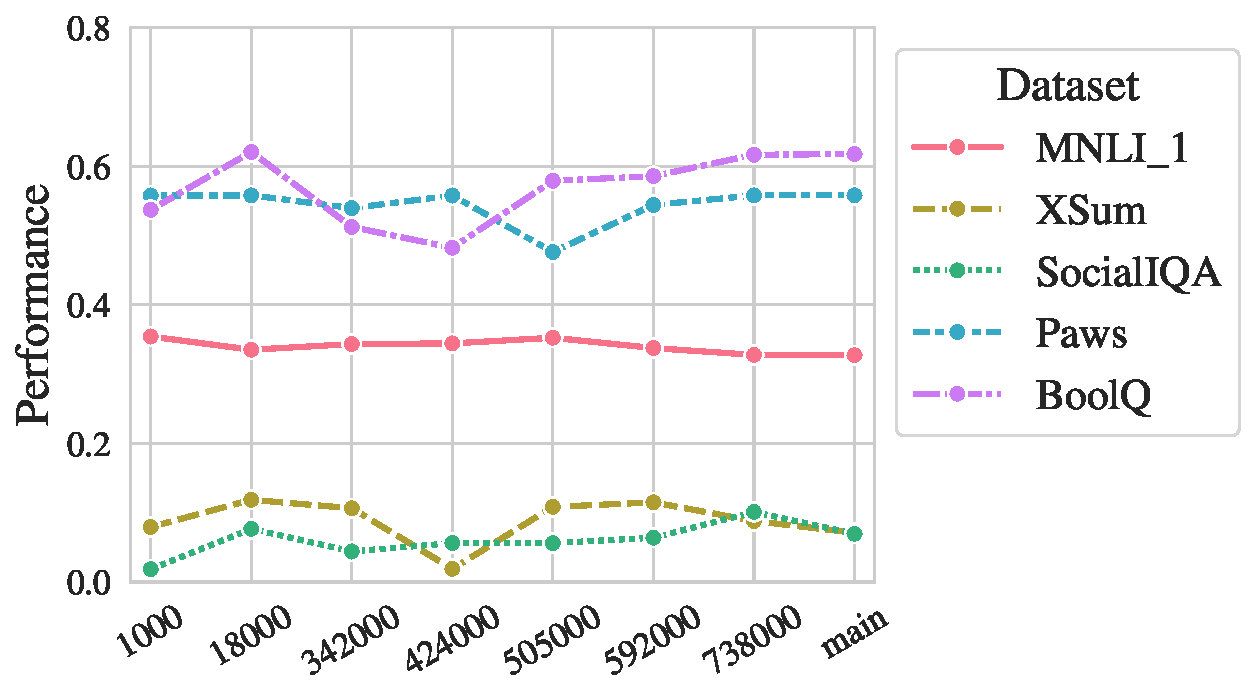
\includegraphics[width=\the\columnwidth]{figures/fig_files/base_notimproving.pdf}
        \caption{Never learned during pre-training.}
        \label{fig:base-eval-b}
    \end{subfigure}
    \caption{Few-shot performance on different pre-training steps.}
    \label{fig:base-eval}
\end{figure*}


\begin{figure}[t!]
    \begin{subfigure}[b]{0.5\textwidth}
    \centering
    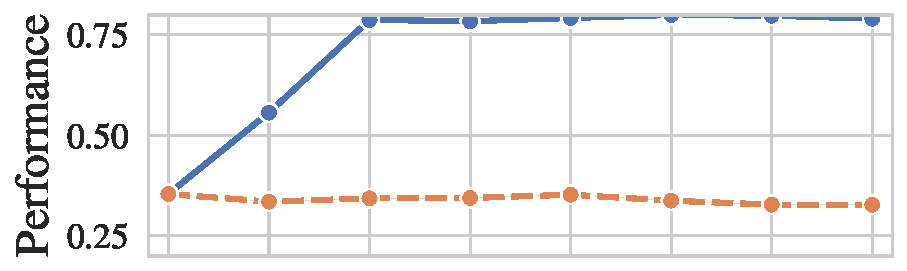
\includegraphics[width=0.8\columnwidth]{figures/fig_files/sft_evalmnli_matched-trainmnli_tight.pdf}
        \caption{MNLI Matched}
        \label{fig:subfig:improve}
    \end{subfigure}%
    \\
    \begin{subfigure}[b]{0.5\textwidth}
        \centering
    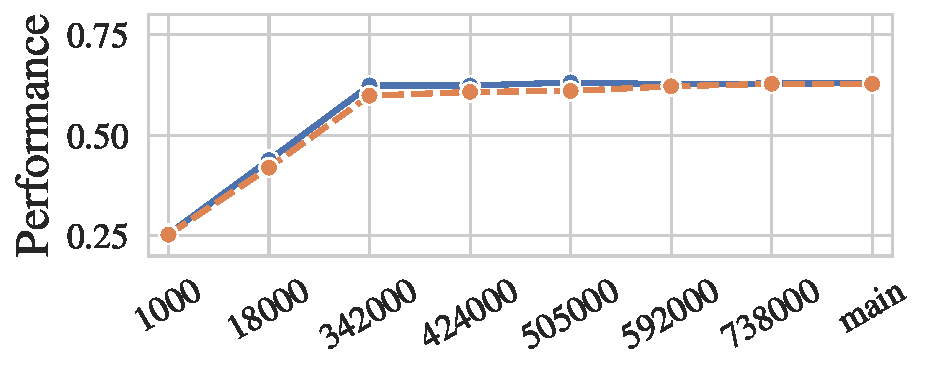
\includegraphics[width=0.8\columnwidth]{figures/fig_files/it_evalhellaswag_tight.pdf}
        \caption{Hellaswag}
        \label{fig:subfig:notimprove}
    \end{subfigure}
    \caption{Example of few-shot performance on different pre-training steps of the models that benefited (\ref{fig:subfig:improve}) and did not benefit from fine-tuning (\ref{fig:subfig:notimprove}). The \textcolor{snsblue}{\textbf{solid blue}} line represents the fine-tuned checkpoint, and the \textcolor{snsorange}{\textbf{dashed orange}} line represents the base checkpoint. The results of all datasets can be found in Figure~\ref{fig:sft-ckpt-perf} and Figure~\ref{fig:it-ckpt-perf}.}
    \label{fig:improve-and-notimprove-example}
\end{figure}
\begin{figure}[t]
    \centering
  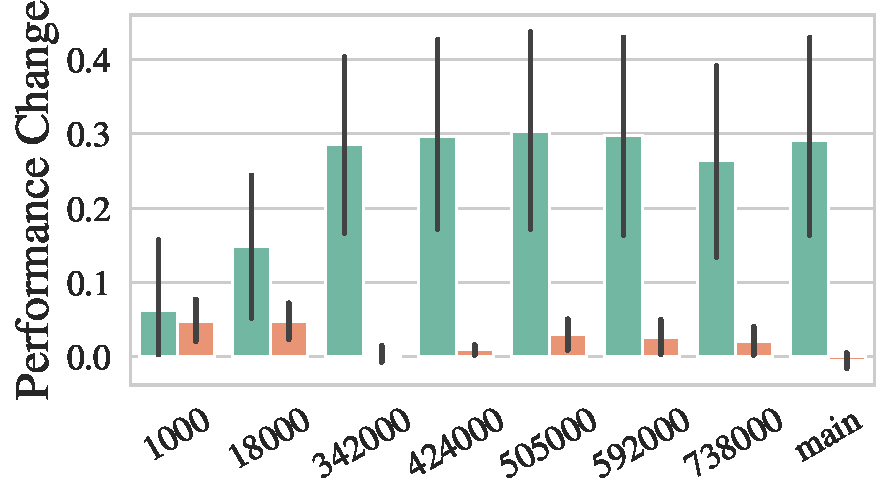
\includegraphics[width=0.84\columnwidth]{figures/fig_files/ptft_comparison_bar.pdf}
  \caption{Amount of performance increase brought by fine-tuning between tasks that model can solve in pre-training (\textcolor{snslightorange}{\textbf{mandarin orange}}) and tasks that the model could not solve until fine-tuning (\textcolor{snsgreen}{\textbf{sage green}}). The exact number of mean increase is shown in Appendix~\ref{sec:app:performance-numbers}.}
  \label{fig:finding:ptftcompare}
\end{figure}


\section{How does the model change across pre-training?}

\label{sec:finding:base-eval}
We begin our evaluation by considering how additional pre-training changes the BASE model. Typically, researchers track the value of the training or held-out loss during training. 
However, performance improvements on downstream tasks do not always follow the same trend with the loss curves \cite{groeneveld2024olmo}.

We evaluate the pre-trained checkpoints with few-shot examples, as models without alignment tend to do poorly in a zero-shot context.
Four shots are randomly sampled from the datasets, which are selected based on the highest performance shot amount reported in \citealp{yang2024unveiling}. 
The model's performance at each pre-training step is reported in Figure~\ref{fig:base-eval}.

Broadly speaking, our results suggest that all datasets fall into one of two groups. 
For the first group of datasets (Figure~\ref{fig:base-eval-a}), although the model shows clear improvement during the early stages of pre-training, performance levels off fairly early on and remains consistent. The dramatic improvements in the early stages of pre-training may result from larger steps in early optimization.
We find improvements stop increasing past step 342,000.
The second group (Figure~\ref{fig:base-eval-a}) shows tasks that are never learned during pre-training. 
Performance remains constant throughout the whole pre-training process. 
These datasets include MNLI, XSum, and BoolQ, and we found no difference between zero-shot and few-shot evaluations.
A natural hypothesis for this finding is potential data contamination in the pre-training data.
However, the evaluation datasets are selected based on the popularity of the task and the content of pre-training data. 
All datasets that experience improvement do not exist in the model's pre-training data \cite{soldaini2024dolma}, while the more likely leaked datasets (MNLI, XSUM) never gain an improvement during the pre-trining process.

Overall, these results reveal an interesting dichotomy. 
Some tasks can be learned during pre-training, while others are not. 
Next, we explore what exactly the model is learning regarding this second group of datasets during pre-training by exploring the fine-tuned models.

\section{Does more pre-training improve fine-tuning?}
\label{sec:finding:PTFT}
\citealp{groeneveld2024olmo} compares OLMo's performance on several tasks before and after fine-tuning the final checkpoint and finds that fine-tuning enables the model to do well on tasks for which the unaligned model does poorly. We observe (\sect{sec:finding:base-eval}) that while some datasets improved 
during pre-training, there is a group of datasets for which a pre-trained model does poorly.
Does the model learn anything that helps solve these tasks, and is fine-tuning required to do well on them? 
Alternatively, does the model learn useful information for these tasks but cannot express it without fine-tuning? In this section, we further explore this dataset dichotomy by examining fine-tuned checkpoints for each of the datasets. 


Our results appear in Figure~\ref{fig:improve-and-notimprove-example} and Figure~\ref{fig:finding:ptftcompare}. First, we consider those datasets where the pre-trained models do well (Figure~\ref{fig:base-eval-a}). 
These datasets do not improve with fine-tuning, suggesting whatever is learned during fine-tuning, which we discuss below, the model already gains the knowledge during pre-training. This effect is observed at all checkpoints; fine-tuning simply does not help.

However, a different story is observed for datasets that are not learned during pre-training. 
For these, fine-tuning yields significant improvements at every model checkpoint, with Figure~\ref{fig:finding:ptftcompare} showing the magnitude of improvement on these datasets compared to no improvement to the datasets already learned during pre-training.
Moreover, earlier checkpoints obtain more substantial gains from fine-tuning than later checkpoints.
The benefit of fine-tuning continues to increase until a certain threshold in pre-training steps is reached (approximately 424,000).

Figure~\ref{fig:improve-and-notimprove-example} shows representative plots comparing the performance of a pre-trained versus fine-tuned model at different checkpoints for two datasets (full list in Appendix~\ref{sec:app:per-ds-ckpt-figures}). 
For Hellaswag (learned during pre-training), fine-tuning does not benefit the model, even during early checkpoints when the model performs poorly on the task. 
Nevertheless, for MNLI (not learned during pre-training), fine-tuning dramatically improves the model. 
Interestingly, later checkpoints achieve better results after fine-tuning, even when the performance of the pre-trained model is unchanged. 
This suggests that the model is, in fact, learning important information during pre-training, but it cannot express that information without fine-tuning.


Our findings suggest that early stopping in pre-training will not be detrimental to downstream fine-tuning performance, and \textbf{the benefits of fine-tuning an LLM could exceed the benefits of continued pretraining}, which sheds light on the potential of cost-effective training paradigm with less pre-training.
However, it is difficult to directly identify such a stopping criteria without fine-tuning intermediate checkpoints; the improvement trend is invisible before fine-tuning the checkpoints.
Future work may reveal other signals of pre-training behavior that correlate with downstream task performance after fine-tuning.
Overall, when resource-intensive pre-trained LLMs are not available, fine-tuning models on models with less pre-training may be a reasonable practical choice for obtaining a high-quality model.


\section{Supervised Fine-Tuning: What does the model learn and forget?}
\label{sec:finding:what}
What exactly is the model learning during fine-tuning such that it shows abilities in pre-trained models for some tasks but provides no benefit for other tasks?
We analyze the supervised fine-tuning process to understand what is learned and what is forgotten. 
Specifically, we explore three dimensions: \textbf{task format, task transfer, and domain knowledge}.


\begin{figure*}[t!]
    \centering
    \begin{subfigure}[b]{0.36\textwidth}
    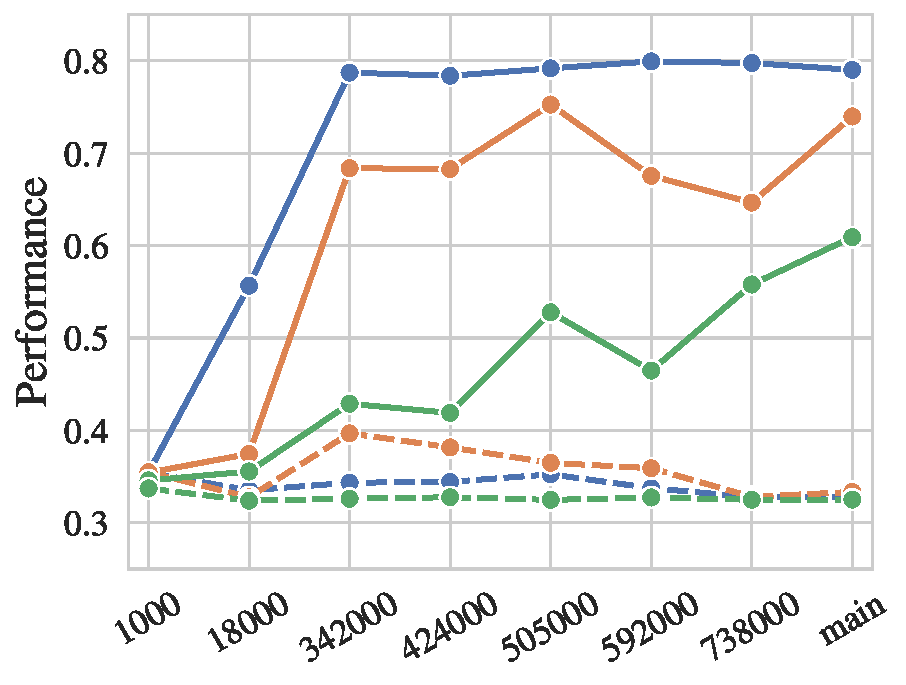
\includegraphics[width=\the\columnwidth]{figures/fig_files/task_format/task_format_evalmnli_matched-trainmnli.pdf}
        \caption{MNLI matched}
    \end{subfigure}%
    ~
    \begin{subfigure}[b]{0.51\textwidth}
    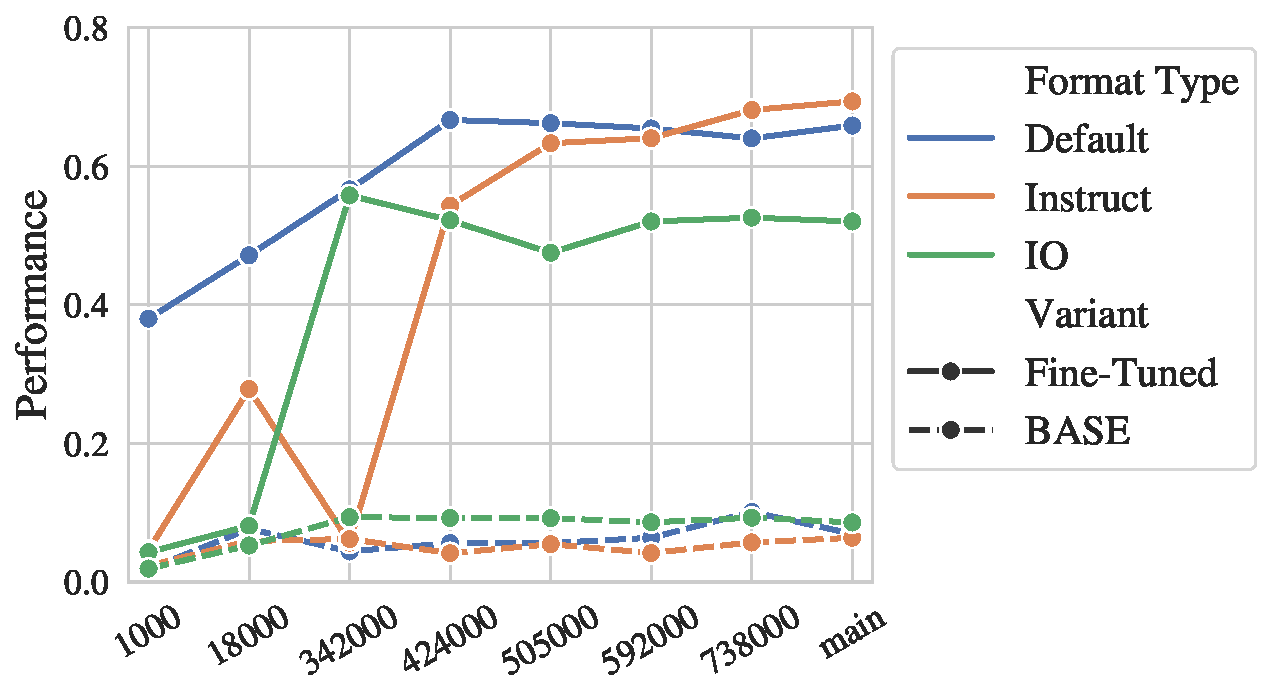
\includegraphics[width=\the\columnwidth]{figures/fig_files/task_format/task_format_evalsocialiqa-trainsocialiqa.pdf}
        \caption{SocialIQa}
    \end{subfigure}%

    \caption {Example of model performance with different task formats. The figure of all datasets can be found in Figure~\ref{fig:app:task_format}. }
  \label{fig:findings:task_format}
\end{figure*}
\subsection{Task Format}
\citealp{sclar2023quantifying} show that LLMs are extremely sensitive to prompt perturbation in few-shot settings. 
More broadly, extensive work on prompt engineering reveals the sensitivity of models to task format.
We hypothesize that fine-tuning fits the model to a specific task format, resulting in higher performance when the evaluation set matches this format. 
To test this hypothesis, we vary the task format to either match the training format, use a different format, or rely on instructions. 
We carefully construct three different prompt formats for the following settings. 1) 
\texttt{Default} is the same format used for training, where we expect the model to benefit from learning the task format;
2) In contrast, \texttt{IO} format reflects a common way of performing supervised fine-tuning by incorporating only unprocessed input and output;
3) \texttt{Instruct} uses a human-readable instruction template to format the input.
Table~\ref{tab:app:promptformat} shows an example of each format.
Checkpoint performance before and after fine-tuning is shown in Figure~\ref{fig:findings:task_format}.

In the early pre-training steps, aligning the task format with fine-tuning data seems to play a crucial role. 
The model does not yet have enough information to overcome the differences between the training and test formats.
However, when fine-tuned on later pre-training checkpoints, the model gradually becomes more flexible with different task formats, suggesting that model sensitivity to prompt formatting observed may be resolvable with more pre-training and a fine-tuning stage. In this view, fine-tuning teaches the model how to format a response for the task.


\subsection{Task Transfer}
Numerous studies examine model forgetting, where further model training causes improvements on some tasks but degradation on others \cite{mehta2023empirical}. 
We evaluate model forgetfulness by examining whether the model does worse on some tasks after fine-tuning for other tasks. 
Specifically, we divide our tasks into two types: classification and generation. 
We notate the training datasets as $D_{T}$ and the evaluation datasets as $D_{E}$. 
We represent the performance of a pre-trained model (BASE) on checkpoint $i$ as ${\text{Perf}}_{BASE}^i(d)$ where an evaluation dataset $d\in D_{E}$, and the performance of the i-th checkpoint fine-tuned on dataset $t \in D_{t}$ be $\text{Perf}_{t}^{i}(d)$. To normalize the effect caused by uneven performance across different datasets, we compute the mean ratio of change (MRC) in performance for each checkpoint as follows.
\begin{equation*}
\centering
    \resizebox{205pt}{!}{$\text{MRC} = \frac{1}{|D_{E}\setminus \{t\}|}\sum \limits_{\forall d \in D_{E}, d \neq t}{\frac{\text{Perf}_{t}^{i}(d) - {\text{Perf}}_{BASE}^i(d)}{\text{Perf}_{BASE}^i(d)}}$} 
\end{equation*}

Models fine-tuned on classification tasks and evaluated on generation tasks decrease on average 61.4\% compared to models that are never fine-tuned.
In contrast, models fine-tuned on generation tasks can still perform the same as the BASE model on classification tasks, with a 0.3\% MRC, which is not statistically significantly different from a 0\% change.
Our findings on all pre-training checkpoints align with the findings of \citet{yang2024unveiling} on the final checkpoint of LLAMA-7B.

Regardless of the pre-training stage, a model can maintain classification abilities when trained for generation, but it loses its generation abilities when trained for classification. 
This is perhaps not surprising given that classification tasks can be seen as a subset of generation, while the reverse is not true. 
The model follows a simplicity bias and thus is more likely to memorize simple classification tasks than generation tasks with an exponentially larger search space.
Additionally, since we evaluate the classification tasks based on the output logits and the base model performs randomly on the classification tasks, it is much easier for the models to maintain the same performance as the BASE models. 
Fine-tuning can cause a model to lose abilities when the desired fine-tuning behavior does not support those abilities.

\begin{figure}[t!]
    \begin{subfigure}[b]{0.5\textwidth}
    \centering
    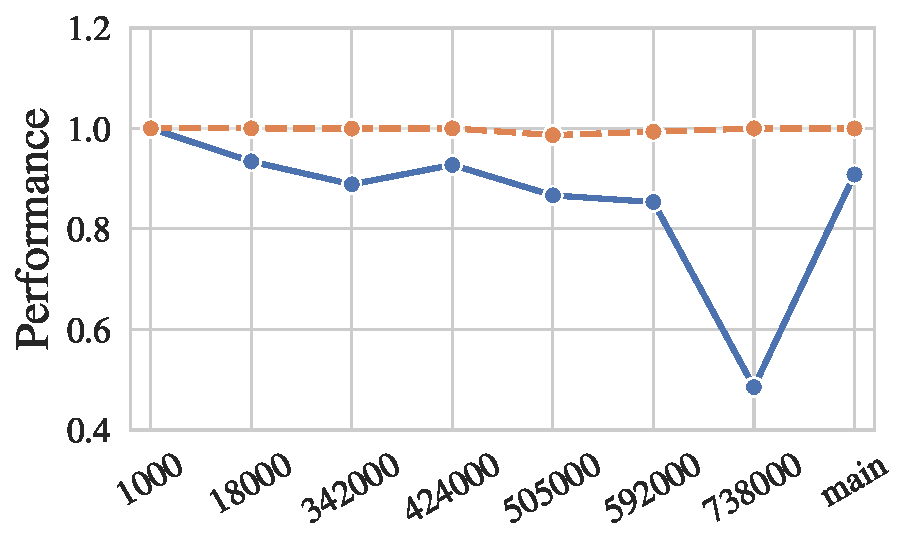
\includegraphics[width=0.7\columnwidth]{figures/fig_files/ood/sft_evalqqp-trainpaws_main_display.pdf}
        \caption{Paws $\rightarrow$ QQP}
        \label{fig:ood:detrimental}
    \end{subfigure}%
    \\
    \begin{subfigure}[b]{0.5\textwidth}
        \centering
    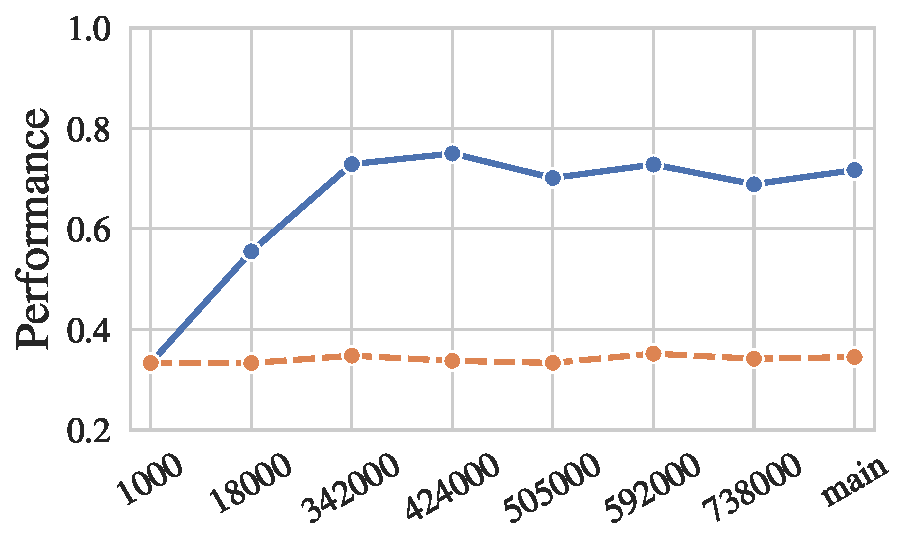
\includegraphics[width=0.7\columnwidth]{figures/fig_files/ood/sft_evalgpt3nli-trainmnli_main_display.pdf}
        \caption{MNLI $\rightarrow$ GPT3NLI}
        \label{fig:ood:beneficial}
    \end{subfigure}
    \caption{Example of out-of-domain performance for fine-tuned models. The \textcolor{snsblue}{\textbf{solid blue}} line represents the fine-tuned checkpoint evaluated on an out-of-domain dataset, and the \textcolor{snsorange}{\textbf{dashed orange}} line represents the base checkpoint where the model is not fine-tuned. Figure~\ref{fig:ood:detrimental} shows an example of fine-tuning hurting OOD performance, while Figure~\ref{fig:ood:beneficial} shows an example of fine-tuning boosting OOD performance as pre-traininng proceeds. }
    \label{fig:findings:ood}
\end{figure}
\begin{figure}[t]
\centering
  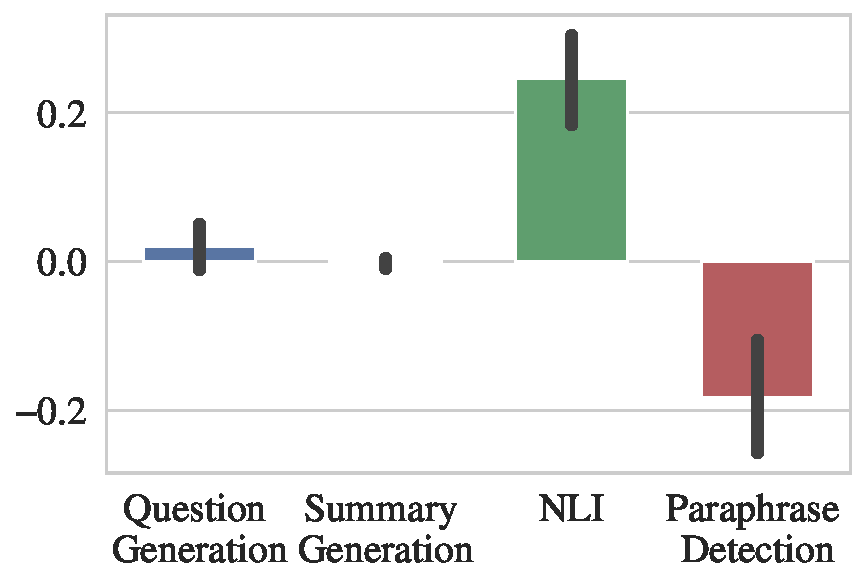
\includegraphics[width=0.65\columnwidth]{figures/fig_files/ood/weighted_ood_transfer_bar.pdf}
  \caption{Ratio of out-of-domain performance change for each task, averaged across checkpoints}
  \label{fig:finding:ood-by-data}
\end{figure}

\subsection{Domain Knowledge}
Finally, we explore how a model's generalization ability is affected by fine-tuning by inspecting whether the model forgets the domain knowledge it had before fine-tuning due to learning other abilities.
An example of OOD model performance is shown in Figure~\ref{fig:findings:ood}, and the mean change ratio by datasets is presented in Figure~\ref{fig:finding:ood-by-data}.

The model does not benefit equally from the in-domain fine-tuning: all NLI datasets experience a boost when fine-tuning on MNLI, while fine-tuning on Paws is detrimental to other paraphrase detection datasets.
This implies that both forgetting and learning are happening: the model learns to perform the task with in-domain knowledge, but it may, in turn, forget information more distant from what is learned in fine-tuning.
Questions remain, however, about whether there are different stages of learning and forgetting during fine-tuning and whether the model picks up different tasks in various stages, which requires further study of fine-tuning dynamics.

Overall, across these three lenses, we find that fine-tuning, although teaches a model how to perform a task, can sacrifice generalization abilities if such ability is not needed for the fine-tuned task. 
For some datasets learned with pre-training alone, the model can easily understand the task format, and the nature of the task is probably supported by the pre-training objective. 
For tasks that can only be learned with subsequent fine-tuning, the model may require additional examples to adapt to different task formats, or the task itself may be inconsistent with the pre-training objective.



\section{Discussion}
Our study uses fine-tuning of pre-training model checkpoints to understand the dynamics of pre-training and fine-tuning on model performance. 
While our insights suggest directions for future work, we note important limitations inherent in our experiments. 
This study considered a single, relatively small LLM on less than a dozen datasets, and still consumed thousands of hours of GPU training time at significant expense. 
Future work needs to confront these issues on larger models and more datasets. We believe our experiments can focus future work on specific experiments with larger models.


{\em Some datasets can be learned without fine-tuning.}
We discover a dichotomy between datasets. 
Some are learned during model pre-training, while others show no improvements during pre-training. 
Furthermore, the datasets learned during pre-training do not benefit from fine-tuning. 
This observation, combined with our study about what is learned during fine-tuning (Section \ref{sec:finding:what}) suggests that some tasks are presented in a manner that aligns with what the model sees during pre-training, and thus fine-tuning provides no additional information. 
While we could identify what about the tasks placed them in the learned or not learnable during pre-training group, it may be possible to format tasks in a manner that better aligns with pre-training and makes them learnable.

{\em Pre-training models can improve in undetectable ways without fine-tuning.}
Some datasets are not learnable during pre-training but benefit significantly from fine-tuning (\sect{sec:finding:base-eval}). 
However, these datasets still benefited from additional pre-training, even though those benefits were not revealed without fine-tuning (\sect{sec:finding:PTFT}).
Clearly, the model is learning important information about the task, even though it cannot express that information.
The identification of a measure available during pre-training that correlated with post-fine-tuning task performance could be used to guide pre-training and produce models that did better post-fine-tuning. 
Perhaps there is a way in which information about these tasks can be included in pre-training, allowing the model to better utilize the massive amount of pre-training data.
For example, early stopping during pre-training could lead to better utilization of limited training resources if we knew when to stop.


{\em Fine-tuning teaches task format but leads to forgetting unused abilities.}
Our results show that fine-tuning guides the model to understand the format and complete a given task. As this information diminishes, the model's overall ability improves. 
However, fine-tuning comes at the expense of other model abilities, such as the capability of performing on tasks or domains that are unrelated to the fine-tuning task. 
This insight can be helpful in our understanding of the multitask abilities of LLMs, where certain tasks can introduce conflicts during multi-task training \cite{mueller-etal-2022-text}.











\section{Conclusion}
Our experiments explore the relationship between fine-tuning and pre-training LLMs.
Our findings span from the latent benefits of pretraining to model learning and forgetting during fine-tuning.
Our results show that the model can rapidly pick up the datasets that it could not solve during fine-tuning with only a small amount of supervision.
In the meantime, we identify the aspects that LLM learns and forgets during supervised fine-tuning: task format, task solution, and domain knowledge.
Overall, our results demonstrate the value of analyzing language model training dynamics, and we would like to call for the release of pre-training checkpoints to aid future studies.

\section*{Limitations}
We discuss the weaknesses and limitations in the following section.

\paragraph{Computing Resource}
Due to computational constraints, we can only conduct experiments on a 1B model and a limited amount of datasets.
The amount of GPU hours spent for each experiment in this study is listed in Table~\ref{app:tab:GPU-hours}.

\paragraph{Availbility of Pre-training Checkpoints}
This study would benefit significantly from including a broader spectrum of models, but the public pre-training checkpoint releases are limited.
Open-source LLMs with intermediate checkpoint release include OLMo \cite{groeneveld2024olmo}, TinyLLAMA, RedPajama-Incite, OpenLM, and Pythia.
After a series of preliminary experiments, we select these models' best-performing and robust families.

\paragraph{Scaling Law}
Recent research shows that the model may resemble emergent capability \cite{wei2022emergent} when scaled to a certain size.
Comparatively, \citealp{hassid2024larger} find that smaller model is capable of outperforming its larger variant when the computing resources is controlled.
To avoid potential confounding factors caused by quantization, our experiments are only conducted on the one-billion model, which may, therefore, conceal the emergent capability brought by larger models while at least giving insights about the potential of small models.

\paragraph{Analysis Protocol}
\citealp{wu2023reasoning} show that the evaluation result may be affected by samples that have been memorized by the model during training instead of revealing the reasoning capability.
The only analysis protocol used is the downstream performance of a trained model.
More investigation should be done into model internals during pre-training dynamics and how they relate to the effects of fine-tuning.

\paragraph{Training Paradigm}
Although multiple tuning strategies exist, to create a fair comparison environment where checkpoints received the same amount of training, models are fine-tuned with a fixed amount of epochs in this work.
On different pre-training stages, the model may converge at a different speed.
Further study can be done to study the effect of pre-training on different fine-tuning methods or fine-tuning dynamics in different pre-training stages.
We only explored the scenario of full-parameter fine-tuning.
Whether parameter-efficient fine-tuning or human preference tuning will lead to a different conclusion also remains an open question.

\paragraph{Randomness}
In this study, we only assess uncertainty with Bootstrap during evaluation.
However, uncertainty may emerge during training, which poses optimizer initialization and data ordering.
Due to the computational constraints, we cannot reduce the randomness factor on this angle.

\section*{Acknowledgments}
The authors thank Saleh Soltan, Niyati Bafna, Fan Bai, Miriam Wanner, Xinbo Wu, Carlos Aguirre for their helpful feedback.

\begin{thebibliography}{88}
    \providecommand{\natexlab}[1]{#1}
    
    \bibitem[{Achiam et~al.(2023)Achiam, Adler, Agarwal, Ahmad, Akkaya, Aleman, Almeida, Altenschmidt, Altman, Anadkat et~al.}]{achiam2023gpt}
    Josh Achiam, Steven Adler, Sandhini Agarwal, Lama Ahmad, Ilge Akkaya, Florencia~Leoni Aleman, Diogo Almeida, Janko Altenschmidt, Sam Altman, Shyamal Anadkat, et~al. 2023.
    \newblock Gpt-4 technical report.
    \newblock \emph{arXiv preprint arXiv:2303.08774}.
    
    \bibitem[{Agirre et~al.(2007)Agirre, M`arquez, and Wicentowski}]{agirre2007semantic}
    Eneko Agirre, Llu'{i}s M`arquez, and Richard Wicentowski, editors. 2007.
    \newblock \emph{Proceedings of the Fourth International Workshop on Semantic Evaluations (SemEval-2007)}.
    \newblock Association for Computational Linguistics, Prague, Czech Republic.
    
    \bibitem[{AI@Meta(2024)}]{llama3modelcard}
    AI@Meta. 2024.
    \newblock \href {https://github.com/meta-llama/llama3/blob/main/MODEL_CARD.md} {Llama 3 model card}.
    
    \bibitem[{Almazrouei et~al.(2023)Almazrouei, Alobeidli, Alshamsi, Cappelli, Cojocaru, Debbah, Goffinet, Hesslow, Launay, Malartic et~al.}]{almazrouei2023falcon}
    Ebtesam Almazrouei, Hamza Alobeidli, Abdulaziz Alshamsi, Alessandro Cappelli, Ruxandra Cojocaru, M{\'e}rouane Debbah, {\'E}tienne Goffinet, Daniel Hesslow, Julien Launay, Quentin Malartic, et~al. 2023.
    \newblock The falcon series of open language models.
    \newblock \emph{arXiv preprint arXiv:2311.16867}.
    
    \bibitem[{Attendu and Corbeil(2023)}]{attendu-corbeil-2023-nlu}
    Jean-michel Attendu and Jean-philippe Corbeil. 2023.
    \newblock \href {https://doi.org/10.18653/v1/2023.sustainlp-1.9} {{NLU} on data diets: Dynamic data subset selection for {NLP} classification tasks}.
    \newblock In \emph{Proceedings of The Fourth Workshop on Simple and Efficient Natural Language Processing (SustaiNLP)}, pages 129--146, Toronto, Canada (Hybrid). Association for Computational Linguistics.
    
    \bibitem[{Bar~Haim et~al.(2006)Bar~Haim, Dagan, Dolan, Ferro, Giampiccolo, Magnini, and Szpektor}]{bar2006second}
    Roy Bar~Haim, Ido Dagan, Bill Dolan, Lisa Ferro, Danilo Giampiccolo, Bernardo Magnini, and Idan Szpektor. 2006.
    \newblock The second {PASCAL} recognising textual entailment challenge.
    
    \bibitem[{Batsuren et~al.(2024)Batsuren, Vylomova, Dankers, Delgerbaatar, Uzan, Pinter, and Bella}]{batsuren2024evaluating}
    Khuyagbaatar Batsuren, Ekaterina Vylomova, Verna Dankers, Tsetsuukhei Delgerbaatar, Omri Uzan, Yuval Pinter, and G{\'a}bor Bella. 2024.
    \newblock Evaluating subword tokenization: Alien subword composition and oov generalization challenge.
    \newblock \emph{arXiv preprint arXiv:2404.13292}.
    
    \bibitem[{Bentivogli et~al.(2009)Bentivogli, Dagan, Dang, Giampiccolo, and Magnini}]{bentivogli2009fifth}
    Luisa Bentivogli, Ido Dagan, Hoa~Trang Dang, Danilo Giampiccolo, and Bernardo Magnini. 2009.
    \newblock The fifth {PASCAL} recognizing textual entailment challenge.
    
    \bibitem[{Bianchi et~al.(2023)Bianchi, Suzgun, Attanasio, R{\"o}ttger, Jurafsky, Hashimoto, and Zou}]{bianchi2023safety}
    Federico Bianchi, Mirac Suzgun, Giuseppe Attanasio, Paul R{\"o}ttger, Dan Jurafsky, Tatsunori Hashimoto, and James Zou. 2023.
    \newblock Safety-tuned llamas: Lessons from improving the safety of large language models that follow instructions.
    \newblock \emph{arXiv preprint arXiv:2309.07875}.
    
    \bibitem[{Biderman et~al.(2023)Biderman, Schoelkopf, Anthony, Bradley, O’Brien, Hallahan, Khan, Purohit, Prashanth, Raff et~al.}]{biderman2023pythia}
    Stella Biderman, Hailey Schoelkopf, Quentin~Gregory Anthony, Herbie Bradley, Kyle O’Brien, Eric Hallahan, Mohammad~Aflah Khan, Shivanshu Purohit, USVSN~Sai Prashanth, Edward Raff, et~al. 2023.
    \newblock Pythia: A suite for analyzing large language models across training and scaling.
    \newblock In \emph{International Conference on Machine Learning}, pages 2397--2430. PMLR.
    
    \bibitem[{Bloom~Str{\"o}m et~al.(2023)Bloom~Str{\"o}m, Slater, Zahran, Berdicevskis, and Schumacher}]{bloom-strom-etal-2023-preparing}
    Eva-Marie Bloom~Str{\"o}m, Onelisa Slater, Aron Zahran, Aleksandrs Berdicevskis, and Anne Schumacher. 2023.
    \newblock \href {https://aclanthology.org/2023.clasp-1.7} {Preparing a corpus of spoken {X}hosa}.
    \newblock In \emph{Proceedings of the 2023 CLASP Conference on Learning with Small Data (LSD)}, pages 62--67, Gothenburg, Sweden. Association for Computational Linguistics.
    
    \bibitem[{Brown et~al.(2020)Brown, Mann, Ryder, Subbiah, Kaplan, Dhariwal, Neelakantan, Shyam, Sastry, Askell et~al.}]{brown2020language}
    Tom Brown, Benjamin Mann, Nick Ryder, Melanie Subbiah, Jared~D Kaplan, Prafulla Dhariwal, Arvind Neelakantan, Pranav Shyam, Girish Sastry, Amanda Askell, et~al. 2020.
    \newblock Language models are few-shot learners.
    \newblock \emph{Advances in neural information processing systems}, 33:1877--1901.
    
    \bibitem[{Chen et~al.(2023)Chen, Schwartz-Ziv, Cho, Leavitt, and Saphra}]{chen2023sudden}
    Angelica Chen, Ravid Schwartz-Ziv, Kyunghyun Cho, Matthew~L Leavitt, and Naomi Saphra. 2023.
    \newblock Sudden drops in the loss: Syntax acquisition, phase transitions, and simplicity bias in mlms.
    \newblock \emph{arXiv preprint arXiv:2309.07311}.
    
    \bibitem[{Chowdhery et~al.(2023)Chowdhery, Narang, Devlin, Bosma, Mishra, Roberts, Barham, Chung, Sutton, Gehrmann et~al.}]{chowdhery2023palm}
    Aakanksha Chowdhery, Sharan Narang, Jacob Devlin, Maarten Bosma, Gaurav Mishra, Adam Roberts, Paul Barham, Hyung~Won Chung, Charles Sutton, Sebastian Gehrmann, et~al. 2023.
    \newblock Palm: Scaling language modeling with pathways.
    \newblock \emph{Journal of Machine Learning Research}, 24(240):1--113.
    
    \bibitem[{Christiano et~al.(2017)Christiano, Leike, Brown, Martic, Legg, and Amodei}]{christiano2017deep}
    Paul~F Christiano, Jan Leike, Tom Brown, Miljan Martic, Shane Legg, and Dario Amodei. 2017.
    \newblock Deep reinforcement learning from human preferences.
    \newblock \emph{Advances in neural information processing systems}, 30.
    
    \bibitem[{Clark et~al.(2019)Clark, Lee, Chang, Kwiatkowski, Collins, and Toutanova}]{clark-etal-2019-boolq}
    Christopher Clark, Kenton Lee, Ming-Wei Chang, Tom Kwiatkowski, Michael Collins, and Kristina Toutanova. 2019.
    \newblock \href {https://doi.org/10.18653/v1/N19-1300} {{B}ool{Q}: Exploring the surprising difficulty of natural yes/no questions}.
    \newblock In \emph{Proceedings of the 2019 Conference of the North {A}merican Chapter of the Association for Computational Linguistics: Human Language Technologies, Volume 1 (Long and Short Papers)}, pages 2924--2936, Minneapolis, Minnesota. Association for Computational Linguistics.
    
    \bibitem[{Clark et~al.(2018)Clark, Cowhey, Etzioni, Khot, Sabharwal, Schoenick, and Tafjord}]{clark2018think}
    Peter Clark, Isaac Cowhey, Oren Etzioni, Tushar Khot, Ashish Sabharwal, Carissa Schoenick, and Oyvind Tafjord. 2018.
    \newblock Think you have solved question answering? try arc, the ai2 reasoning challenge.
    \newblock \emph{arXiv preprint arXiv:1803.05457}.
    
    \bibitem[{Computer(2023)}]{together2023redpajama}
    Together Computer. 2023.
    \newblock \href {https://github.com/togethercomputer/RedPajama-Data} {Redpajama: an open dataset for training large language models}.
    
    \bibitem[{Dagan et~al.(2006)Dagan, Glickman, and Magnini}]{dagan2006pascal}
    Ido Dagan, Oren Glickman, and Bernardo Magnini. 2006.
    \newblock The {PASCAL} recognising textual entailment challenge.
    \newblock In \emph{Machine learning challenges. evaluating predictive uncertainty, visual object classification, and recognising tectual entailment}, pages 177--190. Springer.
    
    \bibitem[{Dettmers et~al.(2022)Dettmers, Lewis, Belkada, and Zettlemoyer}]{dettmers2022gpt3}
    Tim Dettmers, Mike Lewis, Younes Belkada, and Luke Zettlemoyer. 2022.
    \newblock Gpt3. int8 (): 8-bit matrix multiplication for transformers at scale.
    \newblock \emph{Advances in Neural Information Processing Systems}, 35:30318--30332.
    
    \bibitem[{Dettmers et~al.(2024)Dettmers, Pagnoni, Holtzman, and Zettlemoyer}]{dettmers2024qlora}
    Tim Dettmers, Artidoro Pagnoni, Ari Holtzman, and Luke Zettlemoyer. 2024.
    \newblock Qlora: Efficient finetuning of quantized llms.
    \newblock \emph{Advances in Neural Information Processing Systems}, 36.
    
    \bibitem[{Giampiccolo et~al.(2007)Giampiccolo, Magnini, Dagan, and Dolan}]{giampiccolo2007third}
    Danilo Giampiccolo, Bernardo Magnini, Ido Dagan, and Bill Dolan. 2007.
    \newblock The third {PASCAL} recognizing textual entailment challenge.
    \newblock In \emph{Proceedings of the ACL-PASCAL workshop on textual entailment and paraphrasing}, pages 1--9. Association for Computational Linguistics.
    
    \bibitem[{Groeneveld et~al.(2024)Groeneveld, Beltagy, Walsh, Bhagia, Kinney, Tafjord, Jha, Ivison, Magnusson, Wang et~al.}]{groeneveld2024olmo}
    Dirk Groeneveld, Iz~Beltagy, Pete Walsh, Akshita Bhagia, Rodney Kinney, Oyvind Tafjord, Ananya~Harsh Jha, Hamish Ivison, Ian Magnusson, Yizhong Wang, et~al. 2024.
    \newblock Olmo: Accelerating the science of language models.
    \newblock \emph{arXiv preprint arXiv:2402.00838}.
    
    \bibitem[{Gururangan et~al.(2020)Gururangan, Marasovi{\'c}, Swayamdipta, Lo, Beltagy, Downey, and Smith}]{gururangan-etal-2020-dont}
    Suchin Gururangan, Ana Marasovi{\'c}, Swabha Swayamdipta, Kyle Lo, Iz~Beltagy, Doug Downey, and Noah~A. Smith. 2020.
    \newblock \href {https://doi.org/10.18653/v1/2020.acl-main.740} {Don{'}t stop pretraining: Adapt language models to domains and tasks}.
    \newblock In \emph{Proceedings of the 58th Annual Meeting of the Association for Computational Linguistics}, pages 8342--8360, Online. Association for Computational Linguistics.
    
    \bibitem[{Gururangan et~al.(2023)Gururangan, Wortsman, Gadre, Dave, Kilian, Shi, Mercat, Smyrnis, Ilharco, Jordan, Heckel, Dimakis, Farhadi, Shankar, and Schmidt}]{openlm}
    Suchin Gururangan, Mitchell Wortsman, Samir~Yitzhak Gadre, Achal Dave, Maciej Kilian, Weijia Shi, Jean Mercat, Georgios Smyrnis, Gabriel Ilharco, Matt Jordan, Reinhard Heckel, Alex Dimakis, Ali Farhadi, Vaishaal Shankar, and Ludwig Schmidt. 2023.
    \newblock \href {https://github.com/mlfoundations/open_lm/} {{open\_lm}: a minimal but performative language modeling (lm) repository}.
    \newblock GitHub repository.
    
    \bibitem[{Hasan et~al.(2021)Hasan, Bhattacharjee, Islam, Mubasshir, Li, Kang, Rahman, and Shahriyar}]{hasan-etal-2021-xl}
    Tahmid Hasan, Abhik Bhattacharjee, Md.~Saiful Islam, Kazi Mubasshir, Yuan-Fang Li, Yong-Bin Kang, M.~Sohel Rahman, and Rifat Shahriyar. 2021.
    \newblock \href {https://doi.org/10.18653/v1/2021.findings-acl.413} {{XL}-sum: Large-scale multilingual abstractive summarization for 44 languages}.
    \newblock In \emph{Findings of the Association for Computational Linguistics: ACL-IJCNLP 2021}, pages 4693--4703, Online. Association for Computational Linguistics.
    
    \bibitem[{Hassid et~al.(2024)Hassid, Remez, Gehring, Schwartz, and Adi}]{hassid2024larger}
    Michael Hassid, Tal Remez, Jonas Gehring, Roy Schwartz, and Yossi Adi. 2024.
    \newblock The larger the better? improved llm code-generation via budget reallocation.
    \newblock \emph{arXiv preprint arXiv:2404.00725}.
    
    \bibitem[{Hermann et~al.(2015)Hermann, Kocisky, Grefenstette, Espeholt, Kay, Suleyman, and Blunsom}]{hermann2015teaching}
    Karl~Moritz Hermann, Tomas Kocisky, Edward Grefenstette, Lasse Espeholt, Will Kay, Mustafa Suleyman, and Phil Blunsom. 2015.
    \newblock Teaching machines to read and comprehend.
    \newblock \emph{Advances in neural information processing systems}, 28.
    
    \bibitem[{Hoffmann et~al.(2022)Hoffmann, Borgeaud, Mensch, Buchatskaya, Cai, Rutherford, Casas, Hendricks, Welbl, Clark et~al.}]{hoffmann2022training}
    Jordan Hoffmann, Sebastian Borgeaud, Arthur Mensch, Elena Buchatskaya, Trevor Cai, Eliza Rutherford, Diego de~Las Casas, Lisa~Anne Hendricks, Johannes Welbl, Aidan Clark, et~al. 2022.
    \newblock Training compute-optimal large language models.
    \newblock \emph{arXiv preprint arXiv:2203.15556}.
    
    \bibitem[{Hu et~al.(2021)Hu, Shen, Wallis, Allen-Zhu, Li, Wang, Wang, and Chen}]{hu2021lora}
    Edward~J Hu, Yelong Shen, Phillip Wallis, Zeyuan Allen-Zhu, Yuanzhi Li, Shean Wang, Lu~Wang, and Weizhu Chen. 2021.
    \newblock Lora: Low-rank adaptation of large language models.
    \newblock \emph{arXiv preprint arXiv:2106.09685}.
    
    \bibitem[{Hupkes et~al.(2023)Hupkes, Giulianelli, Dankers, Artetxe, Elazar, Pimentel, Christodoulopoulos, Lasri, Saphra, Sinclair et~al.}]{hupkes2023taxonomy}
    Dieuwke Hupkes, Mario Giulianelli, Verna Dankers, Mikel Artetxe, Yanai Elazar, Tiago Pimentel, Christos Christodoulopoulos, Karim Lasri, Naomi Saphra, Arabella Sinclair, et~al. 2023.
    \newblock A taxonomy and review of generalization research in nlp.
    \newblock \emph{Nature Machine Intelligence}, 5(10):1161--1174.
    
    \bibitem[{Ivison et~al.(2023)Ivison, Wang, Pyatkin, Lambert, Peters, Dasigi, Jang, Wadden, Smith, Beltagy et~al.}]{ivison2023camels}
    Hamish Ivison, Yizhong Wang, Valentina Pyatkin, Nathan Lambert, Matthew Peters, Pradeep Dasigi, Joel Jang, David Wadden, Noah~A Smith, Iz~Beltagy, et~al. 2023.
    \newblock Camels in a changing climate: Enhancing lm adaptation with tulu 2.
    \newblock \emph{arXiv preprint arXiv:2311.10702}.
    
    \bibitem[{Jacob et~al.(2018)Jacob, Kligys, Chen, Zhu, Tang, Howard, Adam, and Kalenichenko}]{jacob2018quantization}
    Benoit Jacob, Skirmantas Kligys, Bo~Chen, Menglong Zhu, Matthew Tang, Andrew Howard, Hartwig Adam, and Dmitry Kalenichenko. 2018.
    \newblock Quantization and training of neural networks for efficient integer-arithmetic-only inference.
    \newblock In \emph{Proceedings of the IEEE conference on computer vision and pattern recognition}, pages 2704--2713.
    
    \bibitem[{Jiang et~al.(2023)Jiang, Sablayrolles, Mensch, Bamford, Chaplot, Casas, Bressand, Lengyel, Lample, Saulnier et~al.}]{jiang2023mistral}
    Albert~Q Jiang, Alexandre Sablayrolles, Arthur Mensch, Chris Bamford, Devendra~Singh Chaplot, Diego de~las Casas, Florian Bressand, Gianna Lengyel, Guillaume Lample, Lucile Saulnier, et~al. 2023.
    \newblock Mistral 7b.
    \newblock \emph{arXiv preprint arXiv:2310.06825}.
    
    \bibitem[{Keles and Bayrakl{\i}(2024)}]{keles-bayrakli-2024-llama-2}
    Onur Keles and Omer~Turan Bayrakl{\i}. 2024.
    \newblock \href {https://aclanthology.org/2024.finnlp-1.21} {{LL}a{MA}-2-econ: Enhancing title generation, abstract classification, and academic {Q}{\&}{A} in economic research}.
    \newblock In \emph{Proceedings of the Joint Workshop of the 7th Financial Technology and Natural Language Processing, the 5th Knowledge Discovery from Unstructured Data in Financial Services, and the 4th Workshop on Economics and Natural Language Processing @ LREC-COLING 2024}, pages 212--218, Torino, Italia. ELRA and ICCL.
    
    \bibitem[{Lee et~al.(2023)Lee, Phatale, Mansoor, Lu, Mesnard, Bishop, Carbune, and Rastogi}]{lee2023rlaif}
    Harrison Lee, Samrat Phatale, Hassan Mansoor, Kellie Lu, Thomas Mesnard, Colton Bishop, Victor Carbune, and Abhinav Rastogi. 2023.
    \newblock Rlaif: Scaling reinforcement learning from human feedback with ai feedback.
    \newblock \emph{arXiv preprint arXiv:2309.00267}.
    
    \bibitem[{Li and Liang(2021)}]{li-liang-2021-prefix}
    Xiang~Lisa Li and Percy Liang. 2021.
    \newblock \href {https://doi.org/10.18653/v1/2021.acl-long.353} {Prefix-tuning: Optimizing continuous prompts for generation}.
    \newblock In \emph{Proceedings of the 59th Annual Meeting of the Association for Computational Linguistics and the 11th International Joint Conference on Natural Language Processing (Volume 1: Long Papers)}, pages 4582--4597, Online. Association for Computational Linguistics.
    
    \bibitem[{Lin(2004)}]{lin-2004-rouge}
    Chin-Yew Lin. 2004.
    \newblock \href {https://aclanthology.org/W04-1013} {{ROUGE}: A package for automatic evaluation of summaries}.
    \newblock In \emph{Text Summarization Branches Out}, pages 74--81, Barcelona, Spain. Association for Computational Linguistics.
    
    \bibitem[{Liu et~al.(2021)Liu, Ji, Fu, Tam, Du, Yang, and Tang}]{liu2021p}
    Xiao Liu, Kaixuan Ji, Yicheng Fu, Weng~Lam Tam, Zhengxiao Du, Zhilin Yang, and Jie Tang. 2021.
    \newblock P-tuning v2: Prompt tuning can be comparable to fine-tuning universally across scales and tasks.
    \newblock \emph{arXiv preprint arXiv:2110.07602}.
    
    \bibitem[{Liu et~al.(2023)Liu, Zheng, Du, Ding, Qian, Yang, and Tang}]{liu2023gpt}
    Xiao Liu, Yanan Zheng, Zhengxiao Du, Ming Ding, Yujie Qian, Zhilin Yang, and Jie Tang. 2023.
    \newblock Gpt understands, too.
    \newblock \emph{AI Open}.
    
    \bibitem[{Mehta et~al.(2023)Mehta, Patil, Chandar, and Strubell}]{mehta2023empirical}
    Sanket~Vaibhav Mehta, Darshan Patil, Sarath Chandar, and Emma Strubell. 2023.
    \newblock An empirical investigation of the role of pre-training in lifelong learning.
    \newblock \emph{Journal of Machine Learning Research}, 24(214):1--50.
    
    \bibitem[{Mihaylov et~al.(2018)Mihaylov, Clark, Khot, and Sabharwal}]{mihaylov-etal-2018-suit}
    Todor Mihaylov, Peter Clark, Tushar Khot, and Ashish Sabharwal. 2018.
    \newblock \href {https://doi.org/10.18653/v1/D18-1260} {Can a suit of armor conduct electricity? a new dataset for open book question answering}.
    \newblock In \emph{Proceedings of the 2018 Conference on Empirical Methods in Natural Language Processing}, pages 2381--2391, Brussels, Belgium. Association for Computational Linguistics.
    
    \bibitem[{Min et~al.(2022)Min, Lyu, Holtzman, Artetxe, Lewis, Hajishirzi, and Zettlemoyer}]{min-etal-2022-rethinking}
    Sewon Min, Xinxi Lyu, Ari Holtzman, Mikel Artetxe, Mike Lewis, Hannaneh Hajishirzi, and Luke Zettlemoyer. 2022.
    \newblock \href {https://doi.org/10.18653/v1/2022.emnlp-main.759} {Rethinking the role of demonstrations: What makes in-context learning work?}
    \newblock In \emph{Proceedings of the 2022 Conference on Empirical Methods in Natural Language Processing}, pages 11048--11064, Abu Dhabi, United Arab Emirates. Association for Computational Linguistics.
    
    \bibitem[{Mishra et~al.(2022)Mishra, Khashabi, Baral, and Hajishirzi}]{mishra-etal-2022-cross}
    Swaroop Mishra, Daniel Khashabi, Chitta Baral, and Hannaneh Hajishirzi. 2022.
    \newblock \href {https://doi.org/10.18653/v1/2022.acl-long.244} {Cross-task generalization via natural language crowdsourcing instructions}.
    \newblock In \emph{Proceedings of the 60th Annual Meeting of the Association for Computational Linguistics (Volume 1: Long Papers)}, pages 3470--3487, Dublin, Ireland. Association for Computational Linguistics.
    
    \bibitem[{Mueller et~al.(2022)Mueller, Andrews, and Dredze}]{mueller-etal-2022-text}
    David Mueller, Nicholas Andrews, and Mark Dredze. 2022.
    \newblock \href {https://doi.org/10.18653/v1/2022.findings-emnlp.206} {Do text-to-text multi-task learners suffer from task conflict?}
    \newblock In \emph{Findings of the Association for Computational Linguistics: EMNLP 2022}, pages 2843--2858, Abu Dhabi, United Arab Emirates. Association for Computational Linguistics.
    
    \bibitem[{Narayan et~al.(2018)Narayan, Cohen, and Lapata}]{narayan-etal-2018-dont}
    Shashi Narayan, Shay~B. Cohen, and Mirella Lapata. 2018.
    \newblock \href {https://doi.org/10.18653/v1/D18-1206} {Don{'}t give me the details, just the summary! topic-aware convolutional neural networks for extreme summarization}.
    \newblock In \emph{Proceedings of the 2018 Conference on Empirical Methods in Natural Language Processing}, pages 1797--1807, Brussels, Belgium. Association for Computational Linguistics.
    
    \bibitem[{Narayanan and Aepli(2024)}]{narayanan-aepli-2024-tulu-resource}
    Manu Narayanan and No{\"e}mi Aepli. 2024.
    \newblock \href {https://aclanthology.org/2024.lrec-main.155} {A {T}ulu resource for machine translation}.
    \newblock In \emph{Proceedings of the 2024 Joint International Conference on Computational Linguistics, Language Resources and Evaluation (LREC-COLING 2024)}, pages 1756--1767, Torino, Italia. ELRA and ICCL.
    
    \bibitem[{Olsson et~al.(2022)Olsson, Elhage, Nanda, Joseph, DasSarma, Henighan, Mann, Askell, Bai, Chen et~al.}]{olsson2022context}
    Catherine Olsson, Nelson Elhage, Neel Nanda, Nicholas Joseph, Nova DasSarma, Tom Henighan, Ben Mann, Amanda Askell, Yuntao Bai, Anna Chen, et~al. 2022.
    \newblock In-context learning and induction heads.
    \newblock \emph{arXiv preprint arXiv:2209.11895}.
    
    \bibitem[{Ouyang et~al.(2022)Ouyang, Wu, Jiang, Almeida, Wainwright, Mishkin, Zhang, Agarwal, Slama, Ray et~al.}]{ouyang2022training}
    Long Ouyang, Jeffrey Wu, Xu~Jiang, Diogo Almeida, Carroll Wainwright, Pamela Mishkin, Chong Zhang, Sandhini Agarwal, Katarina Slama, Alex Ray, et~al. 2022.
    \newblock Training language models to follow instructions with human feedback.
    \newblock \emph{Advances in neural information processing systems}, 35:27730--27744.
    
    \bibitem[{Pedregosa et~al.(2011)Pedregosa, Varoquaux, Gramfort, Michel, Thirion, Grisel, Blondel, Prettenhofer, Weiss, Dubourg, Vanderplas, Passos, Cournapeau, Brucher, Perrot, and Duchesnay}]{scikit-learn}
    F.~Pedregosa, G.~Varoquaux, A.~Gramfort, V.~Michel, B.~Thirion, O.~Grisel, M.~Blondel, P.~Prettenhofer, R.~Weiss, V.~Dubourg, J.~Vanderplas, A.~Passos, D.~Cournapeau, M.~Brucher, M.~Perrot, and E.~Duchesnay. 2011.
    \newblock Scikit-learn: Machine learning in {P}ython.
    \newblock \emph{Journal of Machine Learning Research}, 12:2825--2830.
    
    \bibitem[{Perez et~al.(2023)Perez, Ringer, Lukosiute, Nguyen, Chen, Heiner, Pettit, Olsson, Kundu, Kadavath, Jones, Chen, Mann, Israel, Seethor, McKinnon, Olah, Yan, Amodei, Amodei, Drain, Li, Tran-Johnson, Khundadze, Kernion, Landis, Kerr, Mueller, Hyun, Landau, Ndousse, Goldberg, Lovitt, Lucas, Sellitto, Zhang, Kingsland, Elhage, Joseph, Mercado, DasSarma, Rausch, Larson, McCandlish, Johnston, Kravec, El~Showk, Lanham, Telleen-Lawton, Brown, Henighan, Hume, Bai, Hatfield-Dodds, Clark, Bowman, Askell, Grosse, Hernandez, Ganguli, Hubinger, Schiefer, and Kaplan}]{perez-etal-2023-discovering}
    Ethan Perez, Sam Ringer, Kamile Lukosiute, Karina Nguyen, Edwin Chen, Scott Heiner, Craig Pettit, Catherine Olsson, Sandipan Kundu, Saurav Kadavath, Andy Jones, Anna Chen, Benjamin Mann, Brian Israel, Bryan Seethor, Cameron McKinnon, Christopher Olah, Da~Yan, Daniela Amodei, Dario Amodei, Dawn Drain, Dustin Li, Eli Tran-Johnson, Guro Khundadze, Jackson Kernion, James Landis, Jamie Kerr, Jared Mueller, Jeeyoon Hyun, Joshua Landau, Kamal Ndousse, Landon Goldberg, Liane Lovitt, Martin Lucas, Michael Sellitto, Miranda Zhang, Neerav Kingsland, Nelson Elhage, Nicholas Joseph, Noemi Mercado, Nova DasSarma, Oliver Rausch, Robin Larson, Sam McCandlish, Scott Johnston, Shauna Kravec, Sheer El~Showk, Tamera Lanham, Timothy Telleen-Lawton, Tom Brown, Tom Henighan, Tristan Hume, Yuntao Bai, Zac Hatfield-Dodds, Jack Clark, Samuel~R. Bowman, Amanda Askell, Roger Grosse, Danny Hernandez, Deep Ganguli, Evan Hubinger, Nicholas Schiefer, and Jared Kaplan. 2023.
    \newblock \href {https://doi.org/10.18653/v1/2023.findings-acl.847} {Discovering language model behaviors with model-written evaluations}.
    \newblock In \emph{Findings of the Association for Computational Linguistics: ACL 2023}, pages 13387--13434, Toronto, Canada. Association for Computational Linguistics.
    
    \bibitem[{Radford et~al.(2019)Radford, Wu, Child, Luan, Amodei, Sutskever et~al.}]{radford2019language}
    Alec Radford, Jeffrey Wu, Rewon Child, David Luan, Dario Amodei, Ilya Sutskever, et~al. 2019.
    \newblock Language models are unsupervised multitask learners.
    \newblock \emph{OpenAI blog}, 1(8):9.
    
    \bibitem[{Rae et~al.(2021)Rae, Borgeaud, Cai, Millican, Hoffmann, Song, Aslanides, Henderson, Ring, Young et~al.}]{rae2021scaling}
    Jack~W Rae, Sebastian Borgeaud, Trevor Cai, Katie Millican, Jordan Hoffmann, Francis Song, John Aslanides, Sarah Henderson, Roman Ring, Susannah Young, et~al. 2021.
    \newblock Scaling language models: Methods, analysis \& insights from training gopher.
    \newblock \emph{arXiv preprint arXiv:2112.11446}.
    
    \bibitem[{Rafailov et~al.(2024)Rafailov, Sharma, Mitchell, Manning, Ermon, and Finn}]{rafailov2024direct}
    Rafael Rafailov, Archit Sharma, Eric Mitchell, Christopher~D Manning, Stefano Ermon, and Chelsea Finn. 2024.
    \newblock Direct preference optimization: Your language model is secretly a reward model.
    \newblock \emph{Advances in Neural Information Processing Systems}, 36.
    
    \bibitem[{Raffel et~al.(2020)Raffel, Shazeer, Roberts, Lee, Narang, Matena, Zhou, Li, and Liu}]{raffel2020exploring}
    Colin Raffel, Noam Shazeer, Adam Roberts, Katherine Lee, Sharan Narang, Michael Matena, Yanqi Zhou, Wei Li, and Peter~J Liu. 2020.
    \newblock Exploring the limits of transfer learning with a unified text-to-text transformer.
    \newblock \emph{Journal of machine learning research}, 21(140):1--67.
    
    \bibitem[{Riviere et~al.(2024)Riviere, Pathak, Sessa, Hardin, Bhupatiraju, Hussenot, Mesnard, Shahriari, Ram{\'e} et~al.}]{team2024gemma}
    Morgane Riviere, Shreya Pathak, Pier~Giuseppe Sessa, Cassidy Hardin, Surya Bhupatiraju, L{\'e}onard Hussenot, Thomas Mesnard, Bobak Shahriari, Alexandre Ram{\'e}, et~al. 2024.
    \newblock Gemma 2: Improving open language models at a practical size.
    \newblock \emph{arXiv preprint arXiv:2408.00118}.
    
    \bibitem[{Sap et~al.(2019)Sap, Rashkin, Chen, Le~Bras, and Choi}]{sap-etal-2019-social}
    Maarten Sap, Hannah Rashkin, Derek Chen, Ronan Le~Bras, and Yejin Choi. 2019.
    \newblock \href {https://doi.org/10.18653/v1/D19-1454} {Social {IQ}a: Commonsense reasoning about social interactions}.
    \newblock In \emph{Proceedings of the 2019 Conference on Empirical Methods in Natural Language Processing and the 9th International Joint Conference on Natural Language Processing (EMNLP-IJCNLP)}, pages 4463--4473, Hong Kong, China. Association for Computational Linguistics.
    
    \bibitem[{Schulman et~al.(2017)Schulman, Wolski, Dhariwal, Radford, and Klimov}]{schulman2017proximal}
    John Schulman, Filip Wolski, Prafulla Dhariwal, Alec Radford, and Oleg Klimov. 2017.
    \newblock Proximal policy optimization algorithms.
    \newblock \emph{arXiv preprint arXiv:1707.06347}.
    
    \bibitem[{Sclar et~al.(2023)Sclar, Choi, Tsvetkov, and Suhr}]{sclar2023quantifying}
    Melanie Sclar, Yejin Choi, Yulia Tsvetkov, and Alane Suhr. 2023.
    \newblock Quantifying language models' sensitivity to spurious features in prompt design or: How i learned to start worrying about prompt formatting.
    \newblock \emph{arXiv preprint arXiv:2310.11324}.
    
    \bibitem[{Sharma et~al.(2024)Sharma, Keh, Mitchell, Finn, Arora, and Kollar}]{sharma2024critical}
    Archit Sharma, Sedrick Keh, Eric Mitchell, Chelsea Finn, Kushal Arora, and Thomas Kollar. 2024.
    \newblock A critical evaluation of ai feedback for aligning large language models.
    \newblock \emph{arXiv preprint arXiv:2402.12366}.
    
    \bibitem[{Shen et~al.(2024)Shen, Knearem, Ghosh, Alkiek, Krishna, Liu, Ma, Petridis, Peng, Qiwei, Rakshit, Si, Xie, Bigham, Bentley, Chai, Lipton, Mei, Mihalcea, Terry, Yang, Morris, Resnick, and Jurgens}]{shen2024bidirectional}
    Hua Shen, Tiffany Knearem, Reshmi Ghosh, Kenan Alkiek, Kundan Krishna, Yachuan Liu, Ziqiao Ma, Savvas Petridis, Yi-Hao Peng, Li~Qiwei, Sushrita Rakshit, Chenglei Si, Yutong Xie, Jeffrey~P. Bigham, Frank Bentley, Joyce Chai, Zachary Lipton, Qiaozhu Mei, Rada Mihalcea, Michael Terry, Diyi Yang, Meredith~Ringel Morris, Paul Resnick, and David Jurgens. 2024.
    \newblock Towards bidirectional human-ai alignment: A systematic review for clarifications, framework, and future directions.
    \newblock \emph{arXiv preprint arXiv:2406.09264}.
    
    \bibitem[{Singh and Strouse(2024)}]{singh2024tokenization}
    Aaditya~K Singh and DJ~Strouse. 2024.
    \newblock Tokenization counts: the impact of tokenization on arithmetic in frontier llms.
    \newblock \emph{arXiv preprint arXiv:2402.14903}.
    
    \bibitem[{Soldaini et~al.(2024)Soldaini, Kinney, Bhagia, Schwenk, Atkinson, Authur, Bogin, Chandu, Dumas, Elazar et~al.}]{soldaini2024dolma}
    Luca Soldaini, Rodney Kinney, Akshita Bhagia, Dustin Schwenk, David Atkinson, Russell Authur, Ben Bogin, Khyathi Chandu, Jennifer Dumas, Yanai Elazar, et~al. 2024.
    \newblock Dolma: An open corpus of three trillion tokens for language model pretraining research.
    \newblock \emph{arXiv preprint arXiv:2402.00159}.
    
    \bibitem[{Song et~al.(2024)Song, Yu, Li, Yu, Huang, Li, and Wang}]{song2024preference}
    Feifan Song, Bowen Yu, Minghao Li, Haiyang Yu, Fei Huang, Yongbin Li, and Houfeng Wang. 2024.
    \newblock Preference ranking optimization for human alignment.
    \newblock In \emph{Proceedings of the AAAI Conference on Artificial Intelligence}, volume~38, pages 18990--18998.
    
    \bibitem[{Stiennon et~al.(2020)Stiennon, Ouyang, Wu, Ziegler, Lowe, Voss, Radford, Amodei, and Christiano}]{stiennon2020learning}
    Nisan Stiennon, Long Ouyang, Jeffrey Wu, Daniel Ziegler, Ryan Lowe, Chelsea Voss, Alec Radford, Dario Amodei, and Paul~F Christiano. 2020.
    \newblock Learning to summarize with human feedback.
    \newblock \emph{Advances in Neural Information Processing Systems}, 33:3008--3021.
    
    \bibitem[{Su et~al.(2024)Su, Ahmed, Lu, Pan, Bo, and Liu}]{su2024roformer}
    Jianlin Su, Murtadha Ahmed, Yu~Lu, Shengfeng Pan, Wen Bo, and Yunfeng Liu. 2024.
    \newblock Roformer: Enhanced transformer with rotary position embedding.
    \newblock \emph{Neurocomputing}, 568:127063.
    
    \bibitem[{Sun et~al.(2023)Sun, Qi, Zhang, Liu, Wang, and Huang}]{sun-etal-2023-tokenization}
    Kaiser Sun, Peng Qi, Yuhao Zhang, Lan Liu, William Wang, and Zhiheng Huang. 2023.
    \newblock \href {https://doi.org/10.18653/v1/2023.findings-emnlp.887} {Tokenization consistency matters for generative models on extractive {NLP} tasks}.
    \newblock In \emph{Findings of the Association for Computational Linguistics: EMNLP 2023}, pages 13300--13310, Singapore. Association for Computational Linguistics.
    
    \bibitem[{Tian et~al.(2023)Tian, Wang, Chen, and Du}]{tian2023scan}
    Yuandong Tian, Yiping Wang, Beidi Chen, and Simon~S Du. 2023.
    \newblock Scan and snap: Understanding training dynamics and token composition in 1-layer transformer.
    \newblock \emph{Advances in Neural Information Processing Systems}, 36:71911--71947.
    
    \bibitem[{Tirumala et~al.(2022)Tirumala, Markosyan, Zettlemoyer, and Aghajanyan}]{tirumala2022memorization}
    Kushal Tirumala, Aram Markosyan, Luke Zettlemoyer, and Armen Aghajanyan. 2022.
    \newblock Memorization without overfitting: Analyzing the training dynamics of large language models.
    \newblock \emph{Advances in Neural Information Processing Systems}, 35:38274--38290.
    
    \bibitem[{Touvron et~al.(2023)Touvron, Martin, Stone, Albert, Almahairi, Babaei, Bashlykov, Batra, Bhargava, Bhosale et~al.}]{touvron2023llama}
    Hugo Touvron, Louis Martin, Kevin Stone, Peter Albert, Amjad Almahairi, Yasmine Babaei, Nikolay Bashlykov, Soumya Batra, Prajjwal Bhargava, Shruti Bhosale, et~al. 2023.
    \newblock Llama 2: Open foundation and fine-tuned chat models.
    \newblock \emph{arXiv preprint arXiv:2307.09288}.
    
    \bibitem[{Victor et~al.(2022)Victor, Albert, Colin, Stephen, Lintang, Zaid, Antoine, Arnaud, Arun, Manan et~al.}]{victor2022multitask}
    Sanh Victor, Webson Albert, Raffel Colin, Bach Stephen, Sutawika Lintang, Alyafeai Zaid, Chaffin Antoine, Stiegler Arnaud, Raja Arun, Dey Manan, et~al. 2022.
    \newblock Multitask prompted training enables zero-shot task generalization.
    \newblock In \emph{International Conference on Learning Representations}.
    
    \bibitem[{Wang et~al.(2018)Wang, Singh, Michael, Hill, Levy, and Bowman}]{wang-etal-2018-glue}
    Alex Wang, Amanpreet Singh, Julian Michael, Felix Hill, Omer Levy, and Samuel Bowman. 2018.
    \newblock \href {https://doi.org/10.18653/v1/W18-5446} {{GLUE}: A multi-task benchmark and analysis platform for natural language understanding}.
    \newblock In \emph{Proceedings of the 2018 {EMNLP} Workshop {B}lackbox{NLP}: Analyzing and Interpreting Neural Networks for {NLP}}, pages 353--355, Brussels, Belgium. Association for Computational Linguistics.
    
    \bibitem[{Wang et~al.(2024)Wang, Dong, Delalleau, Zeng, Shen, Egert, Zhang, Sreedhar, and Kuchaiev}]{wang2024helpsteer2}
    Zhilin Wang, Yi~Dong, Olivier Delalleau, Jiaqi Zeng, Gerald Shen, Daniel Egert, Jimmy~J. Zhang, Makesh~Narsimhan Sreedhar, and Oleksii Kuchaiev. 2024.
    \newblock Helpsteer2: Open-source dataset for training top-performing reward models.
    \newblock \emph{arXiv preprint arXiv:2406.08673}.
    
    \bibitem[{Wei et~al.(2021)Wei, Bosma, Zhao, Guu, Yu, Lester, Du, Dai, and Le}]{wei2021finetuned}
    Jason Wei, Maarten Bosma, Vincent~Y Zhao, Kelvin Guu, Adams~Wei Yu, Brian Lester, Nan Du, Andrew~M Dai, and Quoc~V Le. 2021.
    \newblock Finetuned language models are zero-shot learners.
    \newblock \emph{arXiv preprint arXiv:2109.01652}.
    
    \bibitem[{Wei et~al.(2022)Wei, Tay, Bommasani, Raffel, Zoph, Borgeaud, Yogatama, Bosma, Zhou, Metzler et~al.}]{wei2022emergent}
    Jason Wei, Yi~Tay, Rishi Bommasani, Colin Raffel, Barret Zoph, Sebastian Borgeaud, Dani Yogatama, Maarten Bosma, Denny Zhou, Donald Metzler, et~al. 2022.
    \newblock Emergent abilities of large language models.
    \newblock \emph{arXiv preprint arXiv:2206.07682}.
    
    \bibitem[{Welbl et~al.(2017)Welbl, Liu, and Gardner}]{welbl2017crowdsourcing}
    Johannes Welbl, Nelson~F Liu, and Matt Gardner. 2017.
    \newblock Crowdsourcing multiple choice science questions.
    \newblock In \emph{Proceedings of the 3rd Workshop on Noisy User-generated Text}, pages 94--106.
    
    \bibitem[{Williams et~al.(2018)Williams, Nangia, and Bowman}]{williams-etal-2018-broad}
    Adina Williams, Nikita Nangia, and Samuel Bowman. 2018.
    \newblock \href {https://doi.org/10.18653/v1/N18-1101} {A broad-coverage challenge corpus for sentence understanding through inference}.
    \newblock In \emph{Proceedings of the 2018 Conference of the North {A}merican Chapter of the Association for Computational Linguistics: Human Language Technologies, Volume 1 (Long Papers)}, pages 1112--1122, New Orleans, Louisiana. Association for Computational Linguistics.
    
    \bibitem[{Wu et~al.(2023)Wu, Qiu, Ross, Aky{\"u}rek, Chen, Wang, Kim, Andreas, and Kim}]{wu2023reasoning}
    Zhaofeng Wu, Linlu Qiu, Alexis Ross, Ekin Aky{\"u}rek, Boyuan Chen, Bailin Wang, Najoung Kim, Jacob Andreas, and Yoon Kim. 2023.
    \newblock Reasoning or reciting? exploring the capabilities and limitations of language models through counterfactual tasks.
    \newblock \emph{arXiv preprint arXiv:2307.02477}.
    
    \bibitem[{Xia et~al.(2024)Xia, Malladi, Gururangan, Arora, and Chen}]{xia2024less}
    Mengzhou Xia, Sadhika Malladi, Suchin Gururangan, Sanjeev Arora, and Danqi Chen. 2024.
    \newblock Less: Selecting influential data for targeted instruction tuning.
    \newblock \emph{arXiv preprint arXiv:2402.04333}.
    
    \bibitem[{Xie et~al.(2021)Xie, Raghunathan, Liang, and Ma}]{xie2021explanation}
    Sang~Michael Xie, Aditi Raghunathan, Percy Liang, and Tengyu Ma. 2021.
    \newblock An explanation of in-context learning as implicit bayesian inference.
    \newblock \emph{arXiv preprint arXiv:2111.02080}.
    
    \bibitem[{Xiong et~al.(2019)Xiong, Wu, Wang, Kulkarni, Yu, Chang, Guo, and Wang}]{xiong-etal-2019-tweetqa}
    Wenhan Xiong, Jiawei Wu, Hong Wang, Vivek Kulkarni, Mo~Yu, Shiyu Chang, Xiaoxiao Guo, and William~Yang Wang. 2019.
    \newblock \href {https://doi.org/10.18653/v1/P19-1496} {{TWEETQA}: A social media focused question answering dataset}.
    \newblock In \emph{Proceedings of the 57th Annual Meeting of the Association for Computational Linguistics}, pages 5020--5031, Florence, Italy. Association for Computational Linguistics.
    
    \bibitem[{Xu et~al.(2024)Xu, Sharaf, Chen, Tan, Shen, Van~Durme, Murray, and Kim}]{xu2024contrastive}
    Haoran Xu, Amr Sharaf, Yunmo Chen, Weiting Tan, Lingfeng Shen, Benjamin Van~Durme, Kenton Murray, and Young~Jin Kim. 2024.
    \newblock Contrastive preference optimization: Pushing the boundaries of llm performance in machine translation.
    \newblock \emph{arXiv preprint arXiv:2401.08417}.
    
    \bibitem[{Yang et~al.(2024)Yang, Zhang, Xu, Lu, Heng, and Lam}]{yang2024unveiling}
    Haoran Yang, Yumeng Zhang, Jiaqi Xu, Hongyuan Lu, Pheng~Ann Heng, and Wai Lam. 2024.
    \newblock Unveiling the generalization power of fine-tuned large language models.
    \newblock \emph{arXiv preprint arXiv:2403.09162}.
    
    \bibitem[{Zellers et~al.(2019)Zellers, Holtzman, Bisk, Farhadi, and Choi}]{zellers-etal-2019-hellaswag}
    Rowan Zellers, Ari Holtzman, Yonatan Bisk, Ali Farhadi, and Yejin Choi. 2019.
    \newblock \href {https://doi.org/10.18653/v1/P19-1472} {{H}ella{S}wag: Can a machine really finish your sentence?}
    \newblock In \emph{Proceedings of the 57th Annual Meeting of the Association for Computational Linguistics}, pages 4791--4800, Florence, Italy. Association for Computational Linguistics.
    
    \bibitem[{Zhang et~al.(2022)Zhang, Roller, Goyal, Artetxe, Chen, Chen, Dewan, Diab, Li, Lin et~al.}]{zhang2022opt}
    Susan Zhang, Stephen Roller, Naman Goyal, Mikel Artetxe, Moya Chen, Shuohui Chen, Christopher Dewan, Mona Diab, Xian Li, Xi~Victoria Lin, et~al. 2022.
    \newblock Opt: Open pre-trained transformer language models.
    \newblock \emph{arXiv preprint arXiv:2205.01068}.
    
    \bibitem[{Zhang et~al.(2019)Zhang, Baldridge, and He}]{zhang-etal-2019-paws}
    Yuan Zhang, Jason Baldridge, and Luheng He. 2019.
    \newblock \href {https://doi.org/10.18653/v1/N19-1131} {{PAWS}: Paraphrase adversaries from word scrambling}.
    \newblock In \emph{Proceedings of the 2019 Conference of the North {A}merican Chapter of the Association for Computational Linguistics: Human Language Technologies, Volume 1 (Long and Short Papers)}, pages 1298--1308, Minneapolis, Minnesota. Association for Computational Linguistics.
    
    \bibitem[{Zhou et~al.(2024)Zhou, Liu, Xu, Iyer, Sun, Mao, Ma, Efrat, Yu, Yu et~al.}]{zhou2024lima}
    Chunting Zhou, Pengfei Liu, Puxin Xu, Srinivasan Iyer, Jiao Sun, Yuning Mao, Xuezhe Ma, Avia Efrat, Ping Yu, Lili Yu, et~al. 2024.
    \newblock Lima: Less is more for alignment.
    \newblock \emph{Advances in Neural Information Processing Systems}, 36.
    
    \bibitem[{Ziegler et~al.(2019)Ziegler, Stiennon, Wu, Brown, Radford, Amodei, Christiano, and Irving}]{ziegler2019fine}
    Daniel~M Ziegler, Nisan Stiennon, Jeffrey Wu, Tom~B Brown, Alec Radford, Dario Amodei, Paul Christiano, and Geoffrey Irving. 2019.
    \newblock Fine-tuning language models from human preferences.
    \newblock \emph{arXiv preprint arXiv:1909.08593}.
    
    \end{thebibliography}
    

\clearpage
\appendix
\appendix

% \section{Claimed Emergent Abilities}
% \label{app:claimed_emergent_abilities}

% We compile the models, tasks and metrics that different papers have claimed reveal emergent abilities of large language models. This list may be incomplete or inaccurate, but represents a good faith attempt to compile this information. Note: quantifying model scale when an ability emerges is complicated by the fact that different papers report model scale differently, either as (a) number of parameters \cite{brown2020language, ganguli2022predictability}, (b) effective number of parameters \cite{srivastava2022beyond} or (c) training FLOPs \cite{wei2022emergent}.

% \begin{table}[h!]
%     \centering
%     \begin{tabular}{|l|c|c|c|}
%     \hline
%         Task & Model Families & Metric & Model Scale at Emergence \\
%         \hline
%         2-Digit Addition \cite{brown2020language} & GPT-3 & Accuracy & 13B Parameters\\
%         2-Digit Subtraction \cite{brown2020language} & GPT-3 & Accuracy & 13B Parameters\\
%         3-Digit Addition \cite{brown2020language, ganguli2022predictability} & GPT-3 & Accuracy & 175B Parameters\\
%         3-Digit Subtraction \cite{brown2020language} & GPT-3 & Accuracy & 175B Parameters\\
%         MMLU \cite{ganguli2022predictability} & GPT-3, Gopher & Accuracy & 200B, 300B Parameters\\
%         Program Synthesis \cite{ganguli2022predictability} & Google Internal & \% Samples Solving Task & 200B Parameters\\
%         Figure of Speech Detection \cite{srivastava2022beyond} & ? & ? & $\sim 10^{11}$ Effective Parameters \\
%         IPA Transliterate \cite{srivastava2022beyond, wei2022emergent} & LaMDA, GPT-3 & BLEU & $\sim 10^{23}, \sim 10^{23}$ Training FLOPs\\
%         Periodic Elements \cite{srivastava2022beyond} & ? & ? & ?\\
%         Modified Arithmetic \cite{srivastava2022beyond, wei2022emergent} & GPT-3, LaMDA & Accuracy & $\sim 10^{23}, \sim 10^{24}$ Training FLOPs\\
%         Repeat Copy Logic \cite{srivastava2022beyond} & ? & ? & $10^{11}$ Effective Parameters\\
%         Word Unscrambling \cite{srivastava2022beyond, wei2022emergent} & LaMDA & Exact Match & $\sim 10^{24}$ Training FLOPs\\
%         Persian QA \cite{wei2022emergent} & PaLM & Exact Match & $\sim 10^{24}$ Training FLOPs\\
%         Truthful QA \cite{wei2022emergent} & Gopher & Accuracy & $\sim 10^{23}$ Training FLOPs\\
%         Grounded Mappings \cite{wei2022emergent} & ? & ? & ?\\
%         Multi-task NLU \cite{wei2022emergent} & ? & ? & ?\\
%         Word in context \cite{wei2022emergent} & ? & ? & $\sim 10^{24}$ Training FLOPs\\
%         \hline
%     \end{tabular}
%     \newline
%     \caption{\textbf{Tasks, model families, metrics and number of parameters for emergent abilities.}}
%     \label{tab:my_label}
% \end{table}


% \section{Exponentiated Negative Cross Entropy Lower Bounds Accuracy}
% \label{app:acc_bound}

% Consider batch size $B$ with length $L$. During training i.e. with teacher-forcing, the per-token accuracy (averaged over batch index $b$ and sequence index $l$) is defined as:
% %
% \begin{align}
%     \text{Acc} &\defeq \frac{1}{B} \sum_b \frac{1}{L} \sum_l p(t_{bl}^* | t_{b, <l}^*)\\
%     &= \frac{1}{BL} \sum_{b, l} p(t_{bl}^* | t_{b, <l}^*)
% \end{align}

% The cross entropy (commonly averaged over the batch) is defined as:
% %
% \begin{align}
%     \mathcal{L}_{CE} &\defeq -\frac{1}{B} \sum_b \log p(t_{b 1}^*, ..., t_{b L}^*)\\
%     &= -\frac{1}{B} \sum_b \log \prod_l p(t_{b l}^*| t_{b, <l}^*)\\
%     &= -\frac{1}{B} \sum_{b, l} \log p(t_{bl}^* | t_{b, <l}^*)
% \end{align}

% To make the comparison between accuracy and cross entropy a little easier, let's normalize the cross entropy by the sequence length:
% %
% \begin{align}
%     \mathcal{L}_{CE/L} &\defeq \frac{1}{L}\mathcal{L}_{CE}\\
%     &=  -\frac{1}{BL} \sum_{b, l} \log p(t_{bl}^* | t_{b, <l}^*)
% \end{align}

% Recall that Jensen's inequality tells us that for any random variable $X$, $\log \mathbb{E}[X] \geq \mathbb{E}[\log X]$. The relationship between sequence-length-normalized cross entropy and accuracy is thus:
% %
% \begin{align}
%     -\mathcal{L}_{CE/L} = \frac{1}{BL} \sum_{b, l} \log p(t_{bl}^* | t_{b <l}^*) &\leq \log \frac{1}{BL} \sum_{b, l}  p(t_{bl}^* | t_{b <l}^*) = \log \text{Acc}\\
%     \exp(- \mathcal{L}_{CE/L}) &\leq \text{Acc}
% \end{align}

% Consequently, we see that driving the cross entropy loss to $0$ necessarily drives the accuracy to $1$.

% TODO: Can we use the second moment method to derive bounds on how (un)likely a subset of tokens are to deviate from the mean?


\section{Approximate Behavior of Metrics on Sequential Data}
\label{app:metric_scaling}

How do different metrics behave when used to measure autoregressive model outputs? Precisely answering this question is tricky and possibly analytically unsolvable, so we provide an approximate answer here.

Notationally, we consider $N$ test data of length $L$ (here, length is measured in tokens) with targets denoted $t_n \defeq (t_{n1}, t_{n2}, ... t_{nL})$, the autoregressive model has a true-but-unknown per-token error probability of $\epsilon \in [0, 1]$ and the model outputs prediction $\hat{t}_n \defeq (\hat{t}_{n1}, \hat{t}_{n2}, ... \hat{t}_{nL})$. This assumes that the model's per-token error probability is constant, which is empirically false, but modeling the complex dependencies of errors is beyond our scope.

\subsection{Per-Token Error Probability is Resolution-Limited}
\label{app:metric_scaling:resolution_limited}

Note that because we have $N$ test data, each of length $L$, our resolution for viewing the per-token error probability $\epsilon$ is limited by $1/NL$. 
Here, resolution refers to ``the smallest interval measurable by a scientific instrument; the resolving power."
To explain what resolution means via an example, suppose one wants to measure a coin's probability of yielding heads.
After a single coin flip, only two outcomes are possible (H, T), so the resolution-limited probability of heads is either $0$ or $1$.
After two coin flips, four outcomes are possible (HH, HT, TH, TT), so the resolution-limited probability of heads is now one of $0, 0.5, 1$.
After $F$ coin flips, we can only resolve the coin's probability of yielding heads up to $1/F$.
Consequently, we introduce a resolution-limited notation:
%
\begin{equation}
    \nint{a}_b \defeq \text{$a$ rounded to the nearest integer multiple of $1/b$}
\end{equation}

\subsection{Token Edit Distance}
\label{app:metric_scaling:token_edit_distance}

We first consider an adaptation of the Levenshtein (string edit) distance for models that function on tokens rather than characters, an adaptation we term the \textit{token edit distance}. The token edit distance between two token sequences $t_n, \hat{t_n}$ is defined as the integer number of additions, deletions or substitutions necessary to transform $t_n$ into $\hat{t}_n$ (or vice versa).

\begin{align}
    \text{Token Edit Distance}(t_n, \hat{t}_n)  &\defeq \text{Num Substitutions} + \text{Num. Additions} + \text{Num. Deletions}\\
    &= \sum_{\ell =1}^L \mathbb{I}[t_{n\ell} \neq \hat{t}_{n\ell}] + \text{Num. Additions} + \text{Num. Deletions}\\
    &\geq \sum_{\ell =1}^L \mathbb{I}[t_{n\ell} \neq \hat{t}_{n\ell}]
\end{align}

The expected token edit distance is therefore:

\begin{align}
    \mathbb{E}[\text{Token Edit Distance}(t_n, \hat{t}_n)] &\geq \mathbb{E}[\sum_{\ell =1}^L \mathbb{I}[t_{n\ell} \neq \hat{t}_{n\ell}]]\\
    &= \sum_{\ell =1}^L p(t_{n\ell} \neq \hat{t}_{n\ell})\\
    &\approx L (1 - \epsilon)
\end{align}

The resolution-limited expected token edit distance is therefore:

\begin{equation}
    \nint{\mathbb{E}[\text{Token Edit Distance}(t_n, \hat{t}_n)]}_{NL} \geq L \Big(1 - \nint{\epsilon}_{NL} \Big)
\end{equation}

From this, we see that the expected token edit distance scales approximately linearly with the resolution-limited per-token probability. The real rate is slightly higher than linear because additions and deletions contribute an additional non-negative cost, but modeling this requires a model of how likely the model is to overproduce or underproduce tokens, which is something we do not currently possess.

\subsection{Accuracy}
\label{app:metric_scaling:accuracy}

\begin{align}
    \text{Accuracy}(t_n, \hat{t}_n) &\defeq \mathbb{I}[\text{No additions}] \, \mathbb{I}[\text{No deletions}] \, \prod_{l=1}^L \mathbb{I}[t_{nl} = \hat{t}_{nl}]\\
    &\approx \prod_{l=1}^L \mathbb{I}[t_{nl} = \hat{t}_{nl}]
\end{align}

As with the Token Edit Distance (App. \ref{app:metric_scaling:accuracy}), we ignore how likely the language model is to overproduce or underproduce tokens because we do not have a good model of this process. Continuing along,

\begin{align}
    \mathbb{E}[\log \text{Accuracy}] &= \sum_l \mathbb{E}[\log \mathbb{I}[t_{nl} = \hat{t}_{nl}]]\\
    &\leq \sum_l \log \mathbb{E}[\mathbb{I}[t_{nl} = \hat{t}_{nl}]]\\
    &\approx L \log (1- \epsilon)
    % \exp(\mathbb{E}[\log \text{Accuracy}]) &= \exp (\sum_l \mathbb{E}[\log \mathbb{I}(t_{nl}, \hat{t}_{nl})])\\
    % &=
\end{align}

Taking an approximation that would make most mathematicians cry:

\begin{align}
    \mathbb{E}[\text{Accuracy}] &\approx \exp(\mathbb{E}[\log \text{Accuracy}])\\
    &= (1 - \epsilon)^L\\
\end{align}

This reveals that accuracy \textbf{approximately} falls geometrically with target token length. The resolution-limited expected accuracy is therefore:

\begin{equation}
    \nint{\mathbb{E}[\text{Accuracy}]}_{NL} = \nint{(1 - \epsilon)^L}_{NL}
\end{equation}

From this we can see that choosing a nonlinear metric like Accuracy is affected significantly more by limited resolution because Accuracy forces one to distinguish quantities that decay rapidly.

\subsection{ROUGE-L-Sum}
\label{app:metric_scaling:rougeLsum}

\begin{figure}
    \centering
    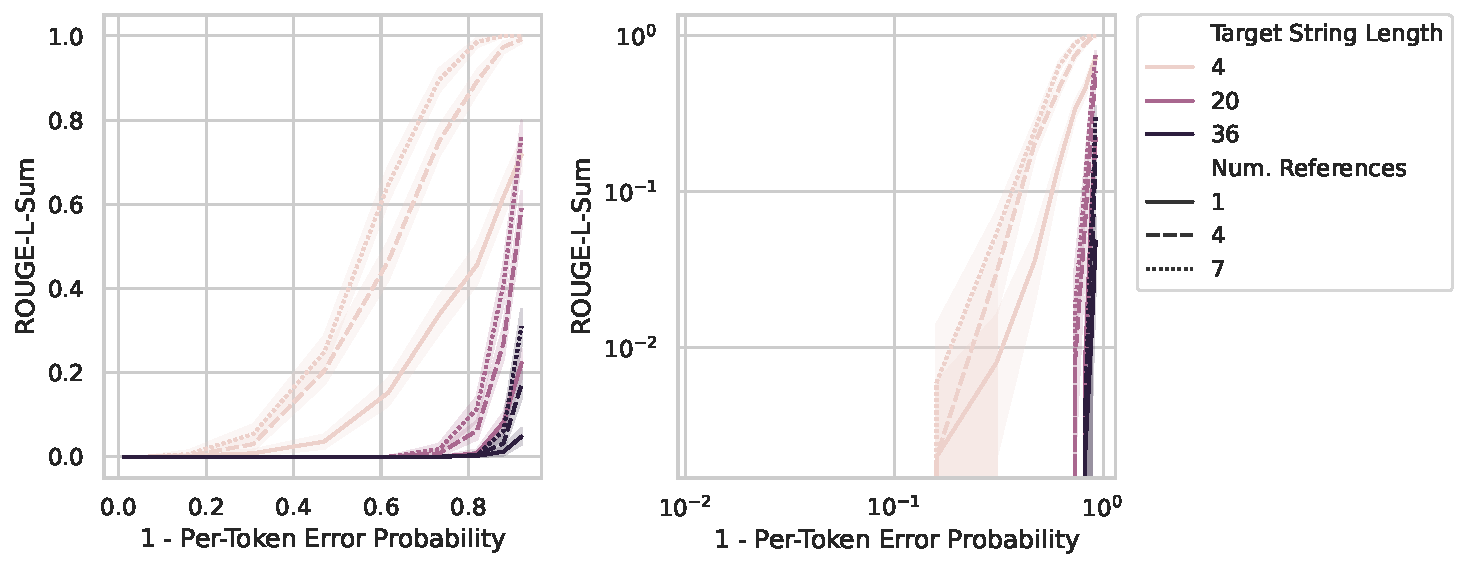
\includegraphics[width=0.95\textwidth]{figures/rouge_understanding/rougeLsum_vs_token_error_prob_scaling_simulation.pdf}
    \caption{\textbf{ROUGE-L-Sum is a sharp metric.} Simulations show that as the per-token error probability slightly increase (e.g. from 0.05 to 0.1), the ROUGE-L-Sum metric sharply falls.}
    \label{fig:app:metric_scaling:rougeLsum}
\end{figure}


Another BIG-Bench metric \cite{srivastava2022beyond} is ROUGE-L-Sum \cite{lin2004rouge}, a metric based on the longest common subsequence (LCS) between two sequences. Section 3.2 of \cite{lin2004rouge} gives the exact definition, but the key property is that ROUGE-L-Sum measures the ``union" LCS, which means ``stitching" together LCSs across the candidate and multiple references. As explained in the original paper: if the candidate sequence is $c = w_1 w_2 w_3 w_4 w_5$, and if there are two reference sequences $r_1 = w_1 w_2 w_6 w_7 w_8$ and $r_2 = w_1 w_3 w_8 w_9 w_5$, then $LCS(r_1, c) = w_1 w_2$ and $LCS(r_2, c) =w_1 w_3 w_5$, then the \textit{union} 
-LCS of $c, r_1, r_2$ is $w_1 w_2 w_3 w_5$, with length 4. Intuitively, this disproportionately benefits models with smaller error rates because their mistakes can be ``stitched" across multiple references; this is confirmed in simulation (Fig. \ref{fig:app:metric_scaling:rougeLsum}).


% \subsection{BLEU}
% \label{app:metric_scaling:bleu}


% \subsection{Emergence does not require on scaling laws: decreasing cross-entropy loss and stricter exact match is all you need }

% The goal of this section is to show that scaling laws are not necessary to create emergence and that many functional forms of the loss are valid as long as the form decreases as some other variable decreases -- say the number of parameters in the model.
% This typically holds in modern machine learning. 
% We do this by considering different functional forms of the cross entropy $CE(N)$, as a function of the number of parameters $N$, and show emergence, i.e. sharpness and unpredictability.
% We illustrate this by showing the programmer can exaggerate the sharpness (and therefore emergence) by implying increasing the exact number of tokens required to get correct in the accuracy, i.e. increasing $L$ in our notation.

% \subsubsection{Argument}

% Recall from section \ref{sec:alt_explanation} the accuracy requiring all $L$ tokens to be correct for a model of size $N$ as a function of cross-entropy $CE(N)$:

% \begin{equation*}
%     \text{Accuracy}(N) \approx p_N(\text{single token correct})^{\text{num. of tokens}} = \exp \Big(- CE(N) \Big)^L
% \end{equation*}

% We plot this equation using three functional forms for a decreasing cross-entropy loss in figure \ref{fig:decreasing_loss_leads_to_emergence_as_L_increases} for increasing values of $L$.
% These increasing values of $L$ induce a sharper -- therefore, seemingly more emergent curve when plotting the accuracy. 
% This means that if the programmer simply requires a stricter accuracy, he can make a perfectly smooth and predictable cross-entropy loss suddenly become sharp and unpredictable, i.e. ``emergent". 
% We show numerically it is independent of the functional form and instead that it only requires the cross-entropy to be decreasing and the accuracy metric to have some non-linear transformation that makes it sharper. 
% Therefore, if one had only tracked the cross-entropy loss instead, one could have had a smooth predictable curve for the models.
% This implies small-scale experimentation is still relevant, and we wish to highly that GPT-4 \cite{gpt4} small-scale experiment in conjunction with scaling loss. 
% We'd like to emphasize that changing the evaluation metric can suddenly induce emergence, and it is not an intrinsic property of the model. 

% %The goal will be to show that if $CE(N)$ decreases with different functional forms that $acc$ is emergent (either sharp or unpredictable).
% % TODO: sharp due to L
% % TODO: unpredictable due to constant and L

% \begin{figure}[htbp]
%   \centering
%   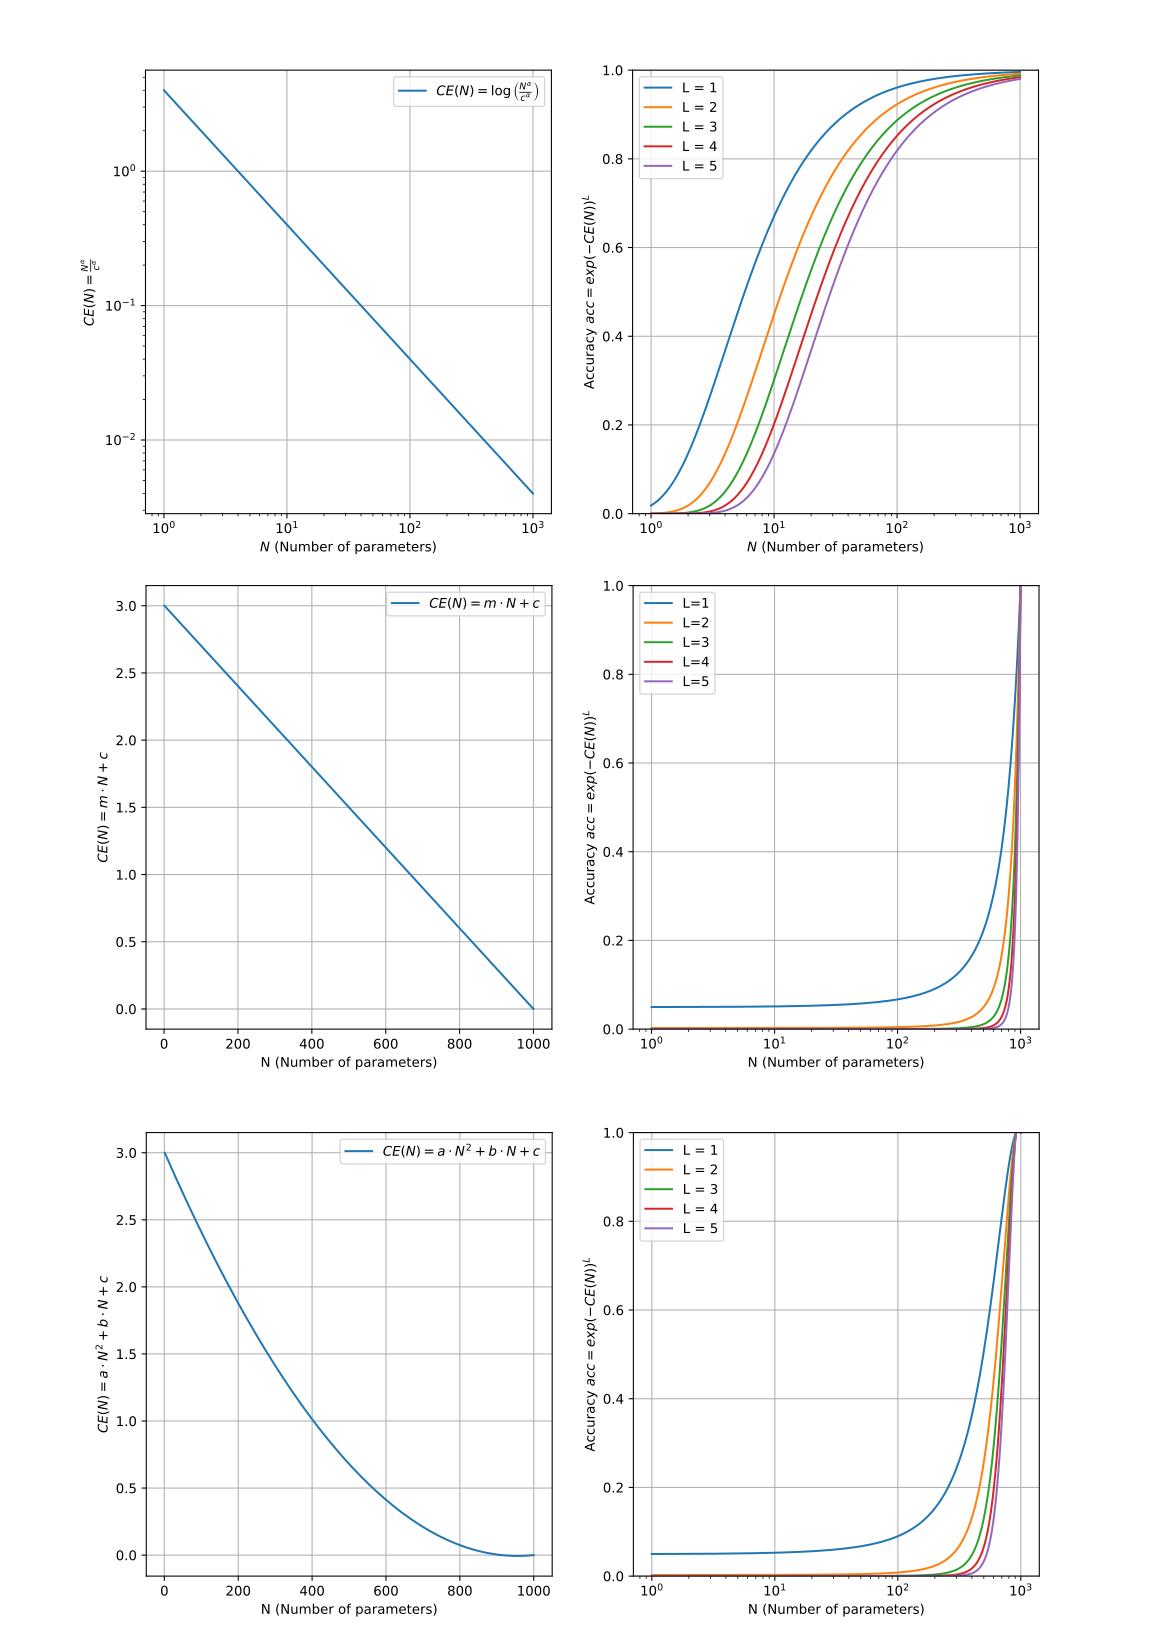
\includegraphics[width=0.8\textwidth]{figures/loss_decreasing_leads_to_emergence/decreasing_loss_leads_to_emergence_as_L_increases.png}
%   \caption{
%   \textbf{Emergence does not depend on scaling laws: any decreasing cross-entropy loss induces apparent emergence as L increases as you require more tokens to be exactly correct, i.e. L increases.}
%   The first row shows the same argument as in the main section, where a decreasing cross-entropy loss as a scaling law induces emergence as $L$ increases.
%   The second row shows the that apparent emergence is induced even when the cross-entropy loss decreases linearly.
%   The third row shows that the apparent emergence is induced when the cross-entropy loss decreases quadratically.
%   Emergence is amplified in this case especially by the increase in sharpness as more tokens are required to be correct. 
%   This means that simply changing the evaluation metric can suddenly induce emergence, and it is not an intrinsic property of the model. 
%   }
%   \label{fig:decreasing_loss_leads_to_emergence_as_L_increases}
% \end{figure}


\section{Inducing Emergent Abilities in Networks on Vision Tasks}
\label{app:sec:inducing_emergence_vision}

\subsection{Emergent Classification of MNIST Handwritten Digits by Convolutional Networks}

\begin{figure}
    \centering
    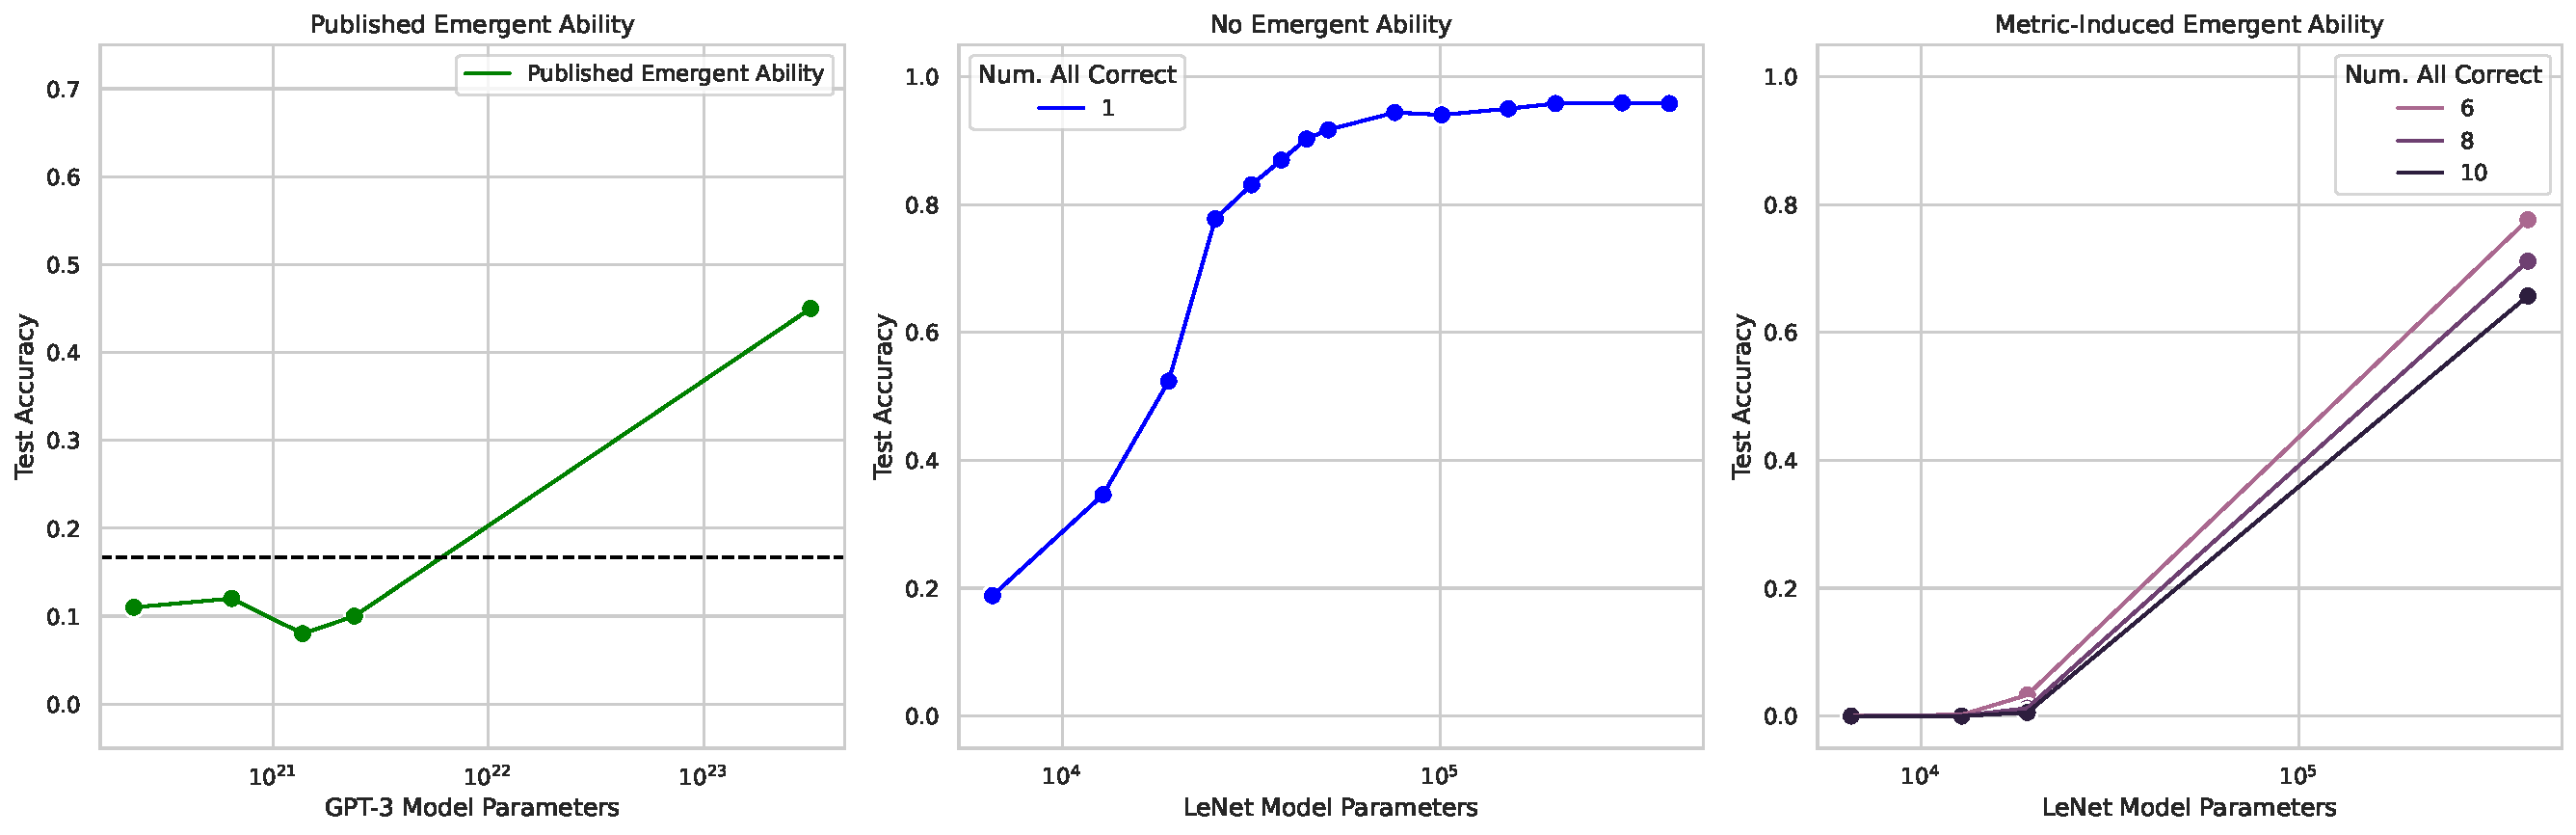
\includegraphics[width=\textwidth]{figures/vision/no_emergence_and_emergence_dataset=mnist.pdf}
    \caption{\textbf{Induced emergent MNIST classification ability in convolutional networks.} (A) A published emergent ability from the BIG-Bench Grounded Mappings task \cite{wei2022emergent}. (B) LeNet trained on MNIST \cite{lecun1998mnist} displays a predictable, commonplace sigmoidal increase in test accuracy as model parameters increase. (C) When accuracy is redefined as correctly classifying $K$ out of $K$ independent test data, this newly defined metric induces a seemingly unpredictable change.}
    \label{fig:vision_mnist}
\end{figure}

We begin by inducing an emergent classification ability in a LeNet convolutional neural network family \cite{lecun1998gradient}, trained on the MNIST handwritten digits dataset \cite{lecun1998mnist}.
This family displays smoothly increasing test accuracy as the number of parameters increase (Fig. \ref{fig:vision_mnist}B).
To emulate the accuracy metric used by emergence papers \cite{ganguli2022predictability, wei2022emergent, srivastava2022beyond}, we use \textit{subset accuracy}: 1 if the network classifies $K$ out of $K$ (independent) test data correctly, 0 otherwise.
Under this definition of accuracy, the model family displays an ``emergent" ability to correctly classify sets of MNIST digits as $K$ increases from $1$ to $5$, especially when combined with sparse sampling of model sizes (Fig. \ref{fig:vision_mnist}C).
This convolutional family's emergent classification ability qualitatively matches published emergent abilities, e.g., at the BIG-Bench Grounded Mappings task \cite{wei2022emergent} (Fig. \ref{fig:vision_mnist}A).

\label{sec:appendix}

\end{document}
